\section{Considerações Iniciais}

%Como apresentado no Capítulo~\ref{chapter:fundamentacao_teorica}, Seção~\ref{sec:refatoracao}, refatorações são técnicas bem conhecidas que auxiliam desenvolvedores durante a reformulação de um determinado sistema com o objetivo de melhorar atributos internos e, ainda, possuem a preocupação de preservar o comportamento original do sistema. Em uma linha de pesquisa paralela, como destacado na Seção~\ref{sec:modernizacaoOrientada_Arquitetura} do Capítulo~\ref{chapter:fundamentacao_teorica}, existe a ADM - uma nova geração de processos para auxiliar e padronizar as atividades da engenharia reversa, utilizando apenas modelos ao invés de código-fonte como os principais artefatos durante o processo de modernização. 
O OMG fornece conceitos gerais para a condução de modernização dirigida a modelos por meio da ADM, porém, o grupo OMG não fornece instruções sobre como criar ou aplicar refatorações em instâncias de seus metamodelos. %Embora a ADM tenha solicitado um \textit{call for proposal}, denominado ADM \textit{Refactoring},\footnote{Até o momento da escrita desta tese a padronização denominada ADM \textit{Refactoring} estava em estágio de discussão. Assim, uma das principais contribuições deste capítulo é auxiliar na criação e adaptação de soluções de refatorações para o metamodelo KDM.} para propor e desenvolver soluções que auxiliem o engenheiro de modernização durante as atividades de refatorações de sistemas com a utilização do metamodelo KDM, até o momento existe, não foi publicado o metamodelo de \textit{refactoring} no site do OMG. 
Assim, existe uma carência de soluções padronizadas e apoios ferramentais durante atividades de refatorações no contexto da ADM. A ausência de instruções claras que guiem o engenheiro de modernização na criação de refatoração para o metamodelo KDM faz com que os engenheiros de modernização sigam procedimentos \textit{ad-hoc} que podem levar a refatorações de baixa qualidade.


%de como criar refatorações já existentes para o metamodelo KDM faz com que engenheiros de modernização criem suas próprias soluções. Usualmente, tais soluções tendem a se tornar proprietárias, o que pode dificultar o reúso, diminuindo a interoperabilidade - um dos principais objetivos da ADM.


%Esta motivação está relaci- onada com a ausência de diretrizes claras que guiem o engenheiro de modernização na criação de refatorações para o metamodelo KDM. A ausência de diretrizes desse tipo faz com que os engenheiros de modernização sigam procedimento ad-hoc que podem levar a refatorações de baixa qualidade;

%O conjunto de refatoração mais conhecido é o catálogo proposto por~\citeonline{Fowler1999}. Esse catálogo foi proposto, primeiramente, para ser utilizado em código-fonte e não em modelos, como a UML e KDM. Embora~\citeonline{Fowler1999} tenha criado um catálogo de refatorações para ser utilizado em código-fonte, mais de 60\% das refatorações (44 de 72) são ilustradas e explicadas utilizando modelos. Tal observação levanta a questão se refatorações \aspas{tradicionais}, ou seja, aquelas aplicadas em código-fonte, podem ser criadas para modelos como o KDM. ~\citeonline{Zhang_2005, Boger_2003} afirmam que algumas refatorações, por exemplo, \texttt{Extract Method}, são mais naturais quando executadas diretamente no código-fonte. Outras refatorações, como \texttt{Rename Class}, \texttt{Pull Up Method}, \texttt{Push Down Method}, etc, podem ser aplicadas tanto em código-fonte, quanto em modelos; já as refatorações que lidam com herança, tais como \texttt{Extract Class}, \texttt{Extract Interface}, \texttt{Replace Inheritance with Delegation}, são mais intuitivas quando aplicadas diretamente em nível de modelo. 

%Embora a refatoração no contexto de modelo tenha alcançado bastante reconhecimento e aceitação na literatura~\cite{Moghadam_2012, Maneerat_2011, Fourati_2011, Einarsson_2012, Steimann_2015, Akiyama_2011, Jensen_2010, Arendt_2012, Millan_2009, Tom_2008_2008}, ainda se fazem necessárias pesquisas nessa área~\cite{durelli_systematic_mapping, revisao_sistematica_uml_refactoring}. Como já salientado até este momento, existe uma ausência de refatorações e de apoios computacionais que auxiliem os engenheiros de modernização e os engenheiros de software a criar, reusar e aplicar refatorações de forma consistente para instâncias do metamodelo KDM. Dessa forma, os engenheiros precisam desenvolver suas próprias refatorações, catálogos e apoios computacionais para refatorar sistemas representados em KDM. Como consequência, essas soluções tornam-se difíceis de ser reutilizadas, diminuindo a interoperabilidade entre as ferramentas de modernização. 

Diante desse contexto, neste capítulo, é apresentada uma abordagem para auxiliar o engenheiro de modernização a criar refatorações para o KDM, a qual conta com um conjunto de passos para auxiliar a criação de refatorações para serem aplicadas em instâncias desse metamodelo. Para ilustrar a utilização dos passos apresentados nesse capítulo, algumas refatorações propostas por~\citeonline{Fowler1999} são criadas para o metamodelo KDM. Utilizando os passos aqui definidos, engenheiros de modernização podem criar refatorações para o metamodelo KDM e facilitar a condução da modernização de um sistema representado como uma instância desse metamodelo~\cite{durelli_catalogo, durelli_VEM_ferramenta}. É importante observar que, neste capítulo, apenas a abordagem para criar refatorações para o metamodelo KDM é apresentada - a preservação de comportamento, pren servação de consistência e sincronização do metamodelo KDM é tratado no módulo de sincronização do apoio computacional KDM-RE, o qual é apresentado no Capítulo~\ref{chapter:ferramenta_kdm_re}  Seção~\ref{sec:modulo_de_sincronizacao_kdm_re}. Dessa forma, observando a Figura~\ref{fig:abordagem_kdm_tese_processo} \ding{202}, nota-se que a abordagem apresentada neste capítulo corresponde a um conjunto de passos para auxiliar o engenheiro de modernização durante a criação de refatorações para o KDM.


%Neste capítulo, também é apresentado um mapeamento entre o paradigma orientado a objetos (POO) e o metamodelo KDM. Por meio desse mapeamento, outros engenheiros de modernização podem adaptar novas refatorações para o metamodelo KDM facilmente. 




%As refatorações apresentadas e adaptadas neste capítulo são baseadas no catálogo de refatoração do~\citeonline{Fowler1999}. O intuito dessas refatorações é facilitar a condução da modernização de um determinado sistema legado representado como uma instância do metamodelo KDM~\cite{durelli_catalogo, durelli_VEM_ferramenta}. Ainda neste capítulo é apresentado um mapeamento entre os conceitos do paradigma orientado a objetos para o metamodelo KDM, assim, engenheiros de modernização podem de forma mais fácil adaptar novas refatorações para o metamodelo KDM. Nota-se que esse capítulo é uma extensão do seguinte artigo: \textit{Towards a Refactoring Catalogue for Knowledge Discovery Metamodel}~\cite{durelli_catalogo}.

%Com o intuito de apresentar e facilitar o entendimento da criação de refatorações para o KDM de uma maneira mais prática, neste capítulo um conjunto de diretrizes são apresentadas. É importante destacar que 

%As refatorações aqui criadas são implementadas com o uso da ATL~\cite{Allilaire_06, Jouault_2005, Jouault_2008} e suas restrições (pre- e pós-condições) são implementadas utilizando OCL. ATL e OCL foram escolhidas nesta tese, pois ambas são linguagens bem conhecidas e amplamente utilizadas na literatura.% Porém, ressalta-se que as refatorações, bem como as pré- e pós-condições podem ser adaptadas com o uso de outras tecnologias, como, por exemplo, \textit{Query/View/Transformation}~\cite{QVT:OMG}, EMF Henshin~\cite{EMF_Henshin}, SmartQVT~\cite{SmartQVT}, ModelMorf~\cite{ModelMorf}, Kermeta~\cite{kermeta}, \textit{Epsilon Transformation Language}~\cite{ETL_eclipse}, OpenArchitectureWare~\cite{OpenArchitectureWare}, VIATRA~\cite{viatra}, AndroMDA~\cite{andromda} e Fujaba \textit{transformations}~\cite{fujaba}.

As demais seções deste capítulo estão organizadas da seguinte forma: Na Seção~\ref{sec:estrategiasParaAdaptarRefatoracoesParaOMetamodeloKDM}, é apresentada a abordagem de criação de refatorações para o metamodelo KDM. Essa abordagem possui seis passos: (\textit{i}) identificar elementos estruturais, (\textit{ii}) identificar operações; (\textit{iii}) implementar refatoração; (\textit{iv}) definir restrições e (\textit{v}) especificar refatoração. Na Seção~\ref{sec:catalogo_refatoracao_kdm}, são apresentados exemplos de uso da abordagem; na Seção~\ref{sec:trabalhos_relacionados_abordagem_criar_kdm}, alguns trabalhos relacionados são descritos; e na Seção~\ref{sec:consideracoes_finais_capitulo_reforacao}, as considerações finais deste capítulo são destacadas. Nota-se que esse capítulo é uma extensão do seguinte artigo: \textit{Towards a Refactoring Catalogue for Knowledge Discovery Metamodel}~\cite{durelli_catalogo}.

%\change{terminar aqui. Deve colocar todas as seções bem escritas.}

\section{Abordagem para Criar Refatorações para o Metamodelo KDM}\label{sec:estrategiasParaAdaptarRefatoracoesParaOMetamodeloKDM}

Nesta seção é apresentada uma abordagem para guiar o engenheiro de modernização durante a criação de refatorações para o metamodelo KDM. %Refatorações em modelos são transformações especiais aplicadas em instâncias de modelos. Esse tipo de refatoração é nova quando comparada com refatorações aplicadas em código-fonte. Dessa forma, com base em informações obtidas das refatorações tradicionais e de abordagens dirigidas por modelos, foi possível definir passos para auxiliar o engenheiro de modernização a criar refatorações para o metamodelo KDM. 
Os passos apresentados neste capítulo utilizam um conjunto de artefatos essenciais para a criação e documentação de refatorações para o contexto da ADM e do KDM. Esses artefatos são descritos a seguir:

\begin{itemize}
\item Mapeamento entre POO e KDM: Esse artefato mapeia os conceitos do POO para o metamodelo KDM (ver Subseção~\ref{sec:mapeamento_POO_e_KDM}). Refatorações são aplicadas em elementos de código, tais como: classes, interfaces, atributos, métodos, etc. Assim, esse artefato é de suma importância para guiar os engenheiros de modernização a identificar quais são as metaclasses em KDM que representam os elementos que serão refatorados;

\item Operações atômicas/compostas: Esse artefato é utilizado para identificar as operações que compõem uma determinada refatoração (ver Subseção~\ref{sec:refatoracao_para_o_metamodelo_kdm}); As refatorações podem ser agrupadas com relação à granularidade: (\textit{i}) operações atômicas e (\textit{ii}) operações compostas;

\item Linguagem de Transformação de Modelo: Aqui \textit{templates} são utilizados como artefatos para guiar a criação de refatorações para o KDM. Refatorações são transformações aplicadas em determinados elementos; no contexto desta tese, em instâncias das metaclasses do KDM. Assim, os elementos estruturais juntamente com a linguagem de transformação de modelo formam o sistema de transformação (ver Subseção~\ref{sec:linguagemDeTransformacaoUtilizada});

\item Linguagem de Restrições: Similarmente, também são utilizados \textit{templates} para guiar a criação de restrições para evitar erros comuns de sintaxe e semântica ao aplicar uma refatoração. Instâncias do metamodelo KDM são entidades não executáveis, assim, se faz necessária a utilização de linguagens de restrições para garantir a correta execução da refatoração antes e depois de sua aplicação (ver Subseção~\ref{sec:linguagem_de_restricao});

\item Documentação: Artefato utilizado para documentar as refatorações. As refatorações podem ser informalmente e formalmente apresentadas e documentadas (ver Subseção~\ref{sec:template_refatoracao});

%\item Gerenciamento de Consistência: Refatorar uma instância de um determinado modelo pode fazer com que ele fique inconsistente. Para preservar a consistência entre as visões da instância do modelo, abordagens de preservação de consistência precisam ser adotadas (ver Capítulo~\ref{chapter:ferramenta_kdm_re} Seção~\ref{sec:modulo_de_sincronizacao_kdm_re});

%\item Apoio Computacional: Implementar um apoio computacional para auxiliar o engenheiro de software a aplicar a refatoração de forma transparente em instâncias do metamodelo KDM (ver Capítulo~\ref{chapter:ferramenta_kdm_re}).
\end{itemize}

No contexto desta tese, cada refatoração criada para o metamodelo KDM consiste em uma transformação que pode ser executada sobre instâncias desse metamodelo. Além disso, as refatorações também possuem pré- e pós-condições que devem ser satisfeitas antes e depois de sua execução. Por exemplo, a refatoração \texttt{Remove ClassUnit} tem como pré-condição a existência de uma instância da metaclasse \texttt{ClassUnit}. %Nota-se que a definição de refatoração no contexto desta tese engloba transformações que preservam o comportamento no contexto de modelos. No contexto do metamodelo KDM, a preservação de comportamento é alcançada por meio do pacote \texttt{Action}, o qual é apresentado no Capítulo~\ref{chapter:fundamentacao_teorica}, Seção~\ref{sec:actionPackage}. 

É importante destacar que, apenas a semântica e a sintaxe são garantidas e preservadas no contexto desta tese após a aplicação de refatorações no KDM. Garantir que a saída/resultado de um sistema representado por meio do KDM não mude após a aplicação de refatorações não é o objetivo desta tese, uma vez que a instância do KDM não pode ser executada. %Diante disso, apenas a semântica e a sintaxe da instância do KDM são preservadas. 
Por exemplo, no que diz respeito à sintaxe, a abordagem restringe que as metaclasses corretas do KDM sejam utilizadas durante a refatoração, por outro lado, a semântica está relacionada com o fato de não existir duas instâncias iguais de uma mesma metaclasse em um mesmo escopo. Dessa forma, a Definição~\ref{def:refatoracao} formaliza refatorações no contexto desta tese:


\begin{definicao}\label{def:refatoracao}
    \textit{Uma refatoração é uma tripla ordenada $Ref = (pre, T, pos)$ em que \textbf{pre} é uma asserção (ou seja, pré-condição), que deve ser verdade em uma determinada instância \textbf{R} do metamodelo KDM, \textbf{T} consiste na transformação do modelo \textbf{R} e \textbf{pos} é a pós-condição a ser aplicada após \textbf{T} ser executada.}
\end{definicao}


Na Figura~\ref{fig:diretrizes_kdm_refatoracao_capitulo}, é exibida uma macrovisão dos elementos/artefatos que são necessários para a criação de refatorações para o KDM, utilizando a notação \sigla{SADT}{\textit{Structured Analysis and Design Technique}}~\cite{Marca_1987}. Como observado, um conjunto de elementos são utilizados como base para a criação de refatorações para o KDM: operações atômicas, \textit{templates}, linguagens de transformações, linguagens de restrições e mapeamento POO - KDM. 

\begin{figure}[h]
	\centering
	% Requires \usepackage{graphicx}
	\caption{Macrovisão para a criação de refatorações para o KDM.}
	\label{fig:diretrizes_kdm_refatoracao_capitulo}
	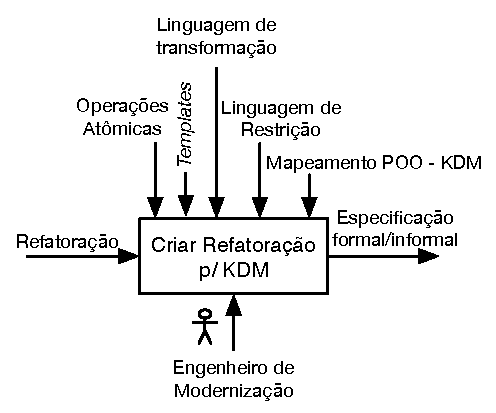
\includegraphics[scale=0.9]{images/novoMacroAbordagemKDMRefactoring2}
	\fautor
\end{figure}


Na Figura~\ref{fig:todos_os_passos_diretrizes}, uma microvisão da Figura~\ref{fig:diretrizes_kdm_refatoracao_capitulo} é apresentada. É visto que a criação de refatorações para o metamodelo KDM possui seis principais passos que o engenheiro de modernização deve seguir. Nas subseções a seguir, esses passos são apresentados. %Gerenciamento de consistência e Apoio computacional são apresentados no Capítulo~\ref{chapter:Abordagem_de_sincronizacao} e Capítulo~\ref{chapter:ferramenta_kdm_re}, respectivamente.


\begin{figure}[h]
	\centering
	% Requires \usepackage{graphicx}
	\caption{Passos para criar refatorações para o KDM.}
	\label{fig:todos_os_passos_diretrizes}
	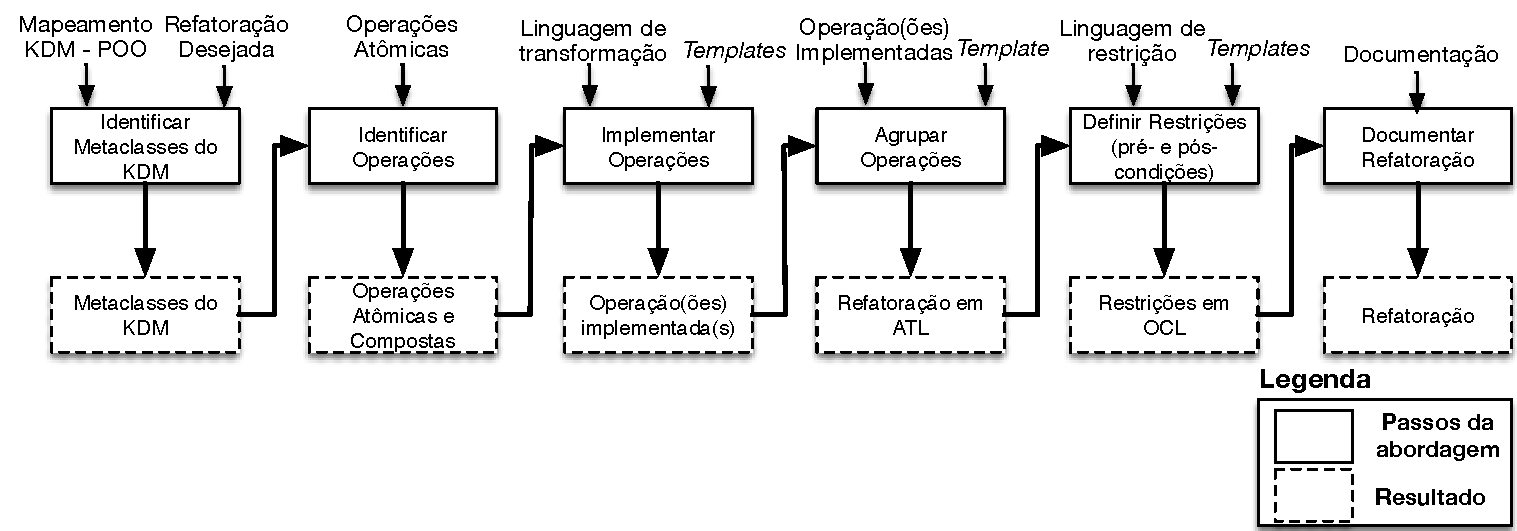
\includegraphics[scale=0.6]{images/Abordagem_Criar_RefatoracaoFinal2}
	\fautor
\end{figure}

\subsection{Identificar Metaclasses do KDM}\label{sec:mapeamento_POO_e_KDM}

Neste passo, o objetivo é identificar as metaclasses do KDM envolvidas na refatoração que será implementada. Os artefatos de entrada para a correta condução deste passo são: (\textit{i}) O Mapeamento KDM - POO e (\textit{ii}) A refatoração desejada. Após a conclusão deste passo, o artefato gerado é uma lista contendo todas as metaclasses que serão utilizadas na criação da refatoração para o KDM.

De acordo com~\citeonline{Zhang_2005, Boger_2003}, um dos maiores desafios quando necessita-se adaptar refatorações para um determinado metamodelo é saber quais são as metaclasses corretas que representam determinadas construções/declarações de um determinado paradigma de programação. É importante identificar se a metaclasse escolhida para fazer a refatoração representa realmente o elemento e o conceito do POO. Dessa forma, antes de realizar a criação de qualquer refatoração para o metamodelo KDM, deve-se, primeiramente, identificar as metaclasses do KDM que têm características similares aos conceitos do POO. 

O artefato Mapeamento KDM - POO é apresentado na Tabela~\ref{tab:mapemanetoEntreOOPeKDM}, onde é possível visualizar as metaclasses do metamodelo KDM que possuem características similares aos conceitos/elementos do POO. Utilizando este artefato, engenheiros de modernização podem identificar as metaclasses necessárias para criar as refatorações para o metamodelo KDM. Assim, qualquer exemplo de refatoração definida para o POO pode ser criada para o metamodelo KDM. Como observado, a Tabela~\ref{tab:mapemanetoEntreOOPeKDM} contém três colunas: \aspas{Elemento do Código-fonte}, \aspas{Pacote::metaclasse do KDM} e \aspas{Descrição}. A primeira coluna informa a construção da linguagem de programação (\textit{statement})e/ou o conceito do POO (pacote, classe, interface, etc.) envolvido na refatoração que se deseja implementar. Em seguida, a coluna \aspas{Pacote::metaclasse do KDM} apresenta a metaclasse responsável por mapear a construção e/ou o conceito do POO e segue o formato \aspas{\textit{Package}::\textit{Meta-class}}. A última coluna, \aspas{Descrição}, possui informações sobre a metaclasse, tais como seu propósito, seus meta-atributos e suas meta-associações.
%\begin{small}
\begin{longtable}[c]{| m{1.9cm} | m{3.57cm}| m{9.3cm} |}
 \caption{Mapeamento entre POO e metaclasses do metamodelo KDM.\label{tab:mapemanetoEntreOOPeKDM}}\\
 
 \hline
 \multicolumn{3}{| c |}{Início da Tabela}\\
 \hline
 Construções de Linguagens OO & Pacote::metaclasse do KDM & Descrição\\
 \hline
 \endfirsthead
 
 \hline
 \multicolumn{3}{|c|}{Continuação da Tabela~\ref{tab:mapemanetoEntreOOPeKDM}}\\
 \hline
 Construções de Linguagens OO & Pacote::metaclasse do KDM & Descrição\\
 \hline
 \endhead
 
 \hline
 \endfoot
 
 \hline
 \multicolumn{3}{| c |}{Fim da Tabela~\ref{tab:mapemanetoEntreOOPeKDM}}\\
 \hline\hline
 \endlastfoot
 
 Pacote & code::Package & A metaclasse \texttt{Package} é um contêiner para elementos de programa, como classes e interfaces. Essa metaclasse contém um meta-atributo, \texttt{name}, que especifica o nome do pacote. Além disso, tal metaclasse possui uma principal meta-associação \texttt{codeElement:AbstractCodeElement[0..*]}, na qual pacotes, classes e interfaces podem ser incluídos. \\ 
\hline
Classe & code::ClassUnit & A metaclasse \texttt{ClassUnit} possui dois principais meta-atributos,  \texttt{name:String} e \texttt{isAbstract:boolean}. O primeiro é utilizado para especificar o nome da classe, o segundo é utilizado para informar se a classe é ou não abstrata. Além disso, essa metaclasse possui três meta-associações: \texttt{attribute:Attribute[0..*]}, \texttt{codeRelation:KDMRelationship[0..*]} e  \texttt{codeElement:AbstractCodeElement[0..*]}. \texttt{attribute} é utilizado para especificar a  visibilidade da classe, ou seja, \textit{public}, \textit{private}, ou \textit{protected}. \texttt{codeRelation}; agrupa todos os relacionamentos que uma determinada classe possui, por exemplo, heranças e associações. \texttt{codeElement} agrupa qualquer metaclasse cujo tipo é uma concretização de \texttt{AbstractCodeElement}, como: \texttt{StorableUnit}, \texttt{MethodUnit}, \texttt{MemberUnit}, etc. \\ 
\hline
Interface & code::InterfaceUnit & A metaclasse \texttt{InterfaceUnit} possui características similares as da metaclasse \texttt{ClassUnit}, porém, não tem o meta-atributo \texttt{isAbstract}, uma vez que todas as interfaces são abstratas por padrão. \\ 
\hline
Atributo & code::StorableUnit & A metaclasse \texttt{StorableUnit} possui dois principais meta-atributos: \texttt{name:String} e \texttt{kind:StorableKind}. Similarmente, essa metaclasse possui dois principais metarrelacionamentos: \texttt{attribute:Attribute[..*]} e \texttt{type:DataType[1]}. \texttt{name} é utilizado para especificar o nome do atributo. \texttt{kind} é uma enumeração utilizada para especificar propriedades do atributo, ou seja, informar se ele é local, global, estático, etc. \texttt{attribute} é utilizado para definir o escopo do atributo, \textit{public}, \textit{private}, ou \textit{protected}. \texttt{type} é utilizado para definir o tipo do atributo.  \\ 
\hline
Método & code::MethodUnit & A metaclasse \texttt{MethodUnit} possui dois principais meta-atributos: \texttt{name:String} e \texttt{kind:MethodKind}. \texttt{name} é utilizado para especificar o nome do método. \texttt{kind} é uma enumeração utilizada para especificar propriedades do método, ou seja, informar se o método é \textit{construtor}, \textit{destructor}, \textit{virtual}, \textit{abstract}, etc. Similarmente, essa metaclasse possui dois principais metarrelacionamentos: \texttt{attribute:Attribute[..*]}, \texttt{codeElement:AbstractCodeElement[0..*]}. \texttt{attribute} é utilizado para definir o escopo do método - informar ele é \textit{public}, \textit{private}, ou \textit{protected}. \texttt{codeElement} é utilizado para agrupar declarações internas do método, ou seja, assinatura do método, bloco do método, etc.\\ 
\hline
Assinatura do Método & code::Signature & A metaclasse \texttt{Signature} possui um principal meta-atributo, \texttt{name:String}, o qual é utilizado para especificar o nome do método. Além disso, essa metaclasse contém um principal metarrelacionamento denominado \texttt{parameterUnit:ParameterUnit[..*]}, que é utilizado para especificar os parâmetros que o método possui.\\ 
\hline
Bloco do Método & action::BlockUnit & A metaclasse \texttt{BlockUnit} representa blocos lógicos e físicos relacionados, por exemplo, com blocos de instruções \textit{if}, \textit{for}, \textit{while}, etc. Possui um metarrelacionamento denominado \texttt{codeElement:AbstractCodeElement[0..*]} que é utilizado para agrupar quaisquer instruções lógicas ou físicas.\\ 
\hline
Parâmetro & code::ParameterUnit & A metaclasse \texttt{ParameterUnit} pode representar o nome, o tipo e a posição dos parâmetros em uma assinatura de método, além de permitir o tipo de parâmetro (valor ou referência). Essa metaclasse contém dois principais meta-atributos: \texttt{name:String} e \texttt{kind:ParameterKind}. O primeiro meta-atributo representa o nome do parâmetro e o segundo meta-atributo é uma enumeração para especificar o tipo de parâmetro (valor ou referência). Além disso, \texttt{ParameterUnit} possui o meta-relacionamento \texttt{type:DataType[1]} para especificar o tipo do parâmetro; esse tipo pode ser tipos primitivos ou outros tipos.\\ 
\hline
Associação & code::HasType & A metaclasse \texttt{HasType} representa uma relação semântica entre um elemento de dados e seu tipo. Essa meta-calsse possui dois principais metarrelacionamentos: \texttt{from:CodeItem} e \texttt{to:DataType}.\\ 
\hline
Herança \texttt{extends} & code::Extends & A metaclasse \texttt{Extends} representa relação semântica de herança entre duas \texttt{ClassUnits} ou duas \texttt{InterfaceUnits}. Essa relação semântica é representada por dois metarrelacionamentos: \texttt{from:DataType} e \texttt{to:DataType}.\\ 
\hline
Herança \texttt{implements} & code::Implements & A metaclasse \texttt{Implements} representa relação semântica de herança entre uma \texttt{ClassUnit} e uma \texttt{InterfaceUnit}. Similarmente a metaclasse \texttt{Extends}, a relação semântica é representada por dois metarrelacionamentos: \texttt{from:DataType} e \texttt{to:DataType}.\\ 
\hline
\textit{if}, \textit{for}, \textit{while}, etc & action::ActionElement & A metaclasse \texttt{ActionElement} representa instruções e declarações de uma determinada linguagem de programação, ou seja, pode ser utilizada para representar ramificações, iterações, etc. \texttt{ActionElement} possui um meta-atributo principal denominado \texttt{kind:String}, que representa qual tipo de instrução que a metaclasse está representando. Essa metaclasse possui dois metarrelacionamentos: \texttt{codeElement:AbstractCodeElement[0..*]} e \texttt{actionRelation:ActionRelationship[0..*]}.\\ 
\hline
 \end{longtable}
%\end{small}

%Na Tabela~\ref{tab:mapemanetoEntreOOPeKDM}, é possível ver a relação existente entre as construções de linguagens OO, bem como algumas instruções de linguagens de programação e algumas metaclasses do metamodelo KDM. Para atender aos objetivos deste trabalho, a Tabela~\ref{tab:mapemanetoEntreOOPeKDM} apresenta apenas as principais metaclasses do KDM.%, uma vez que seria inviável mapear todas as noventa metaclasses do metamodelo KDM.

Como apresentado na Tabela~\ref{tab:mapemanetoEntreOOPeKDM}, algumas metaclasses podem ser diretamente mapeadas com elementos do POO, tais como: classes (\texttt{ClassUnit}), interfaces (\texttt{InterfaceUnit}), atributos (\texttt{StorableUnit}), métodos (\texttt{MethodUnit}), etc. Entretanto, como o KDM é um metamodelo independente de plataforma para representar de forma genérica todas as abstrações e paradigmas de programação, algumas construções de programação não possuem uma metaclasse particular. Por exemplo, iterações e ramificações em KDM são representadas utilizando a mesma metaclasse \texttt{ActionElement}. Esse mapeamento ocorre pois o KDM define uma metaclasse genérica para especificar ramificações e iterações para preservar a independência de plataforma; seria inviável para o metamodelo definir metaclasses específicas para representar ramificações e iterações, uma vez que cada linguagem de programação possui uma determinada particularidade. Para que o mapeamento fique o mais genérico e independente de plataforma possível, a metaclasse \texttt{ActionElement} utiliza o meta-atributo \texttt{kind}, que possui os seguintes valores: \textit{variable declaration}, \textit{if}, \textit{for}, \textit{while}, etc.

Com a utilização da Tabela~\ref{tab:mapemanetoEntreOOPeKDM}, o engenheiro de modernização pode identificar as metaclasses do KDM que serão utilizadas para implementar a refatoração. %É importante identificar previamente qual metaclasse do KDM será utilizada durante a refatoração - com isso, o engenheiro pode criar e implementar a refatoração como apresentado na Seção~\ref{sec:linguagemDeTransformacaoUtilizada}. 
Por exemplo, suponha que o engenheiro de modernização almeje criar a refatoração \texttt{Rename Method}. Dessa forma, utilizando a Tabela~\ref{tab:mapemanetoEntreOOPeKDM} pode-se observar qual é a metaclasse em KDM que representa métodos (métodos em KDM são representados por instâncias da metaclasse \texttt{MethodUnit}), assim, a refatoração torna-se \texttt{Rename MethodUnit}. Suponha também que a refatoração \texttt{Extract Class} também será criada para o KDM. De acordo com~\citeonline{Fowler1999}, uma nova classe deve ser criada e em seguida deve-se mover atributos e métodos para essa nova classe - note que as construções de linguagens OO para a refatoração \texttt{Extract Class} são: classe, atributo e método. Assim, por meio do artefato Mapeamento KDM - POO descrito na Tabela~\ref{tab:mapemanetoEntreOOPeKDM} é possível identificar que as metaclasses \texttt{ClassUnit}, \texttt{StorableUnit} e \texttt{MethodUnit} deverão ser utilizadas para criar a refatoração \texttt{Extract ClassUnit}. Adicionalmente, por meio da Tabela~\ref{tab:mapemanetoEntreOOPeKDM}, é possível identificar todos os relacionamentos que as as metaclasses possuem, os quais podem ser úteis durante a implementação da refatoração.


\subsection{Identificar Operações}\label{sec:refatoracao_para_o_metamodelo_kdm}

Neste passo, o engenheiro de modernização deve identificar quais operações são utilizadas na refatoração que será criada para o KDM. Os artefatos de entrada para a correta execução deste passo são um conjunto de operações atômicas. Como saída deste passo, uma lista é criada, a qual contém um conjunto de operações que serão utilizadas para implementar a refatoração.

%Após identificar todos os elementos estruturais e detectar o mapeamento entre POO e o metamodelo KDM, o próximo passo é determinar as operações que compõem a refatoração a ser criada. Como já salientado, no contexto desta tese, todas refatorações são transformações realizadas em instâncias do KDM. Desse modo, 
As refatorações podem ser agrupadas no nível de sua granularidade. As granularidades podem ser definidas em dois níveis de operações: (\textit{i}) operações atômicas e (\textit{ii}) operações compostas. As granularidades definidas como operações atômicas podem ser especificadas por meio de operações primitivas, que são executadas na instância do metamodelo KDM. Tais operações primitivas são descritas no artefato Operações Atômicas, o qual é apresentado na Tabela~\ref{tab:artefates_atomics_operation}. As operações atômicas e seus efeitos são ilustradas na Figura~\ref{fig:operacoes_atomicas_figuras}\footnote{Para exemplificar o funcionamento das operações atômicas no KDM, diagramas de classes da UML foram utilizados.}.


\begin{table}[h]
\centering
\caption{Operações Atômicas utilizadas para criar refatorações para o KDM.}
\label{tab:artefates_atomics_operation}
\begin{tabular}{|c|m{11.5cm}|}
\hline
\multicolumn{1}{|l|}{Operações Atômicas} & \multicolumn{1}{c|}{Descrição} \\ \hline
\texttt{add}                                      & Qualquer operação que adicione uma instância de uma metaclasse do metamodelo KDM (ver Tabela~\ref{tab:mapemanetoEntreOOPeKDM}). Por exemplo, na Figura~\ref{fig:operacoes_atomicas_figuras}~\ding{202} a operação \texttt{add} está adicionando uma instância de \texttt{ClassUnit} no pacote \aspas{P1};          \\ \hline
\texttt{delete}                                   & Qualquer operação que remove uma instância de uma metaclasse do metamodelo KDM (ver Tabela~\ref{tab:mapemanetoEntreOOPeKDM}). Por exemplo, na Figura~\ref{fig:operacoes_atomicas_figuras}~\ding{203} a operação \texttt{delete} remove a instância da metaclasse \texttt{ClassUnit} do pacote \aspas{P1};           \\ \hline
\texttt{change}                                   & Qualquer operação que altere um valor de um meta-atributo de uma metaclasse do metamodelo KDM (ver Tabela~\ref{tab:mapemanetoEntreOOPeKDM}); Por exemplo, na Figura~\ref{fig:operacoes_atomicas_figuras} \ding{204} a operação \texttt{change} está alterando o meta-atributo \texttt{name} da metaclasse \texttt{StorableUnit}; \texttt{name} para \texttt{addrs}. Além disso, a visibilidade da metaclasse \texttt{StorableUnit} também é alterada de \texttt{private} para \texttt{public}, no diagrama \aspas{-} representa a visibilidade \texttt{private} e \aspas{+} representa \texttt{public}.          \\ \hline
\end{tabular}
\end{table}


%escolher qual refatoração criar. Dessa forma, nesta seção algumas refatorações propostas por~\citeonline{Fowler1999} foram escolhidas para serem adaptadas para o contexto do metamodelo KDM. As refatorações propostas por~\citeonline{Fowler1999} foram escolhidas para serem adaptas para o contexto do metamodelo KDM uma vez que são bem conhecidas, básicas e de baixa granularidade. As refatorações adaptadas seguem a mesma convenção de nomenclatura definida por~\citeonline{Fowler1999}. Porém, os nomes de algumas refatorações foram alteradas para indicar o metamodelo KDM como seu novo domínio de aplicação, por exemplo, \texttt{MoveMethod} torna-se \texttt{MoveMethodUnit} e \texttt{MoveAttribute} torna-se \texttt{MoveStorableUnit}, etc. 

%No contexto desta Tese todas as refatorações são transformações que são realizadas em uma instância do metamodelo KDM. Assim, as refatorações podem ser agrupadas em nível de sua granularidade. As granularidades podem ser definidas em dois níveis de operações: (\textit{i}) operações atômicas e (\textit{ii}) operações compostas. As granularidades definidas como operações atômicas podem ser especificadas por meio de operações primitivas que são executadas na instância do metamodelo KDM. Tais operações primitivas são listadas a seguir:

\begin{figure}[h]
	\centering
	% Requires \usepackage{graphicx}
	\caption{Operações atômicas para o KDM.}
	\label{fig:operacoes_atomicas_figuras}
	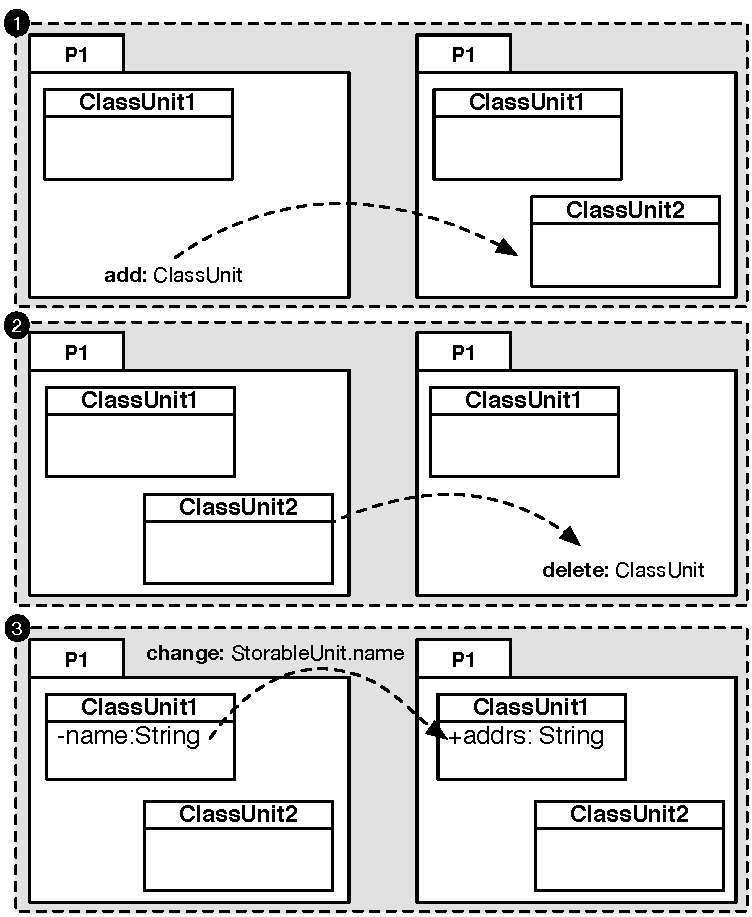
\includegraphics[scale=0.7]{images/identificarOperacoesFig2}
	\fautor
\end{figure}

\begin{comment}

\begin{itemize}
\item \texttt{add}: qualquer operação que adicione uma instância de uma metaclasse do metamodelo KDM (ver Tabela~\ref{tab:mapemanetoEntreOOPeKDM}). Por exemplo, na Figura~\ref{fig:operacoes_atomicas_figuras} \ding{202} a operação \texttt{add} está adicionando uma instância de \texttt{ClassUnit} no pacote \aspas{P1};
\item \texttt{delete}: qualquer operação que remove uma instância de uma metaclasse do metamodelo KDM (ver Tabela~\ref{tab:mapemanetoEntreOOPeKDM}). Por exemplo, na Figura~\ref{fig:operacoes_atomicas_figuras} \ding{203} a operação \texttt{delete} remove a instância da metaclasse \texttt{ClassUnit} do pacote \aspas{P1};
\item \texttt{change}: qualquer operação que altere um valor de um meta-atributo de uma metaclasse do metamodelo KDM (ver Tabela~\ref{tab:mapemanetoEntreOOPeKDM}); Por exemplo, na Figura~\ref{fig:operacoes_atomicas_figuras} \ding{204} a operação \texttt{change} está alterando o meta-atributo \texttt{name} da metaclasse \texttt{StorableUnit}; \texttt{name} para \texttt{addrs}. Além disso, a visibilidade da metaclasse \texttt{StorableUnit} também é alterada de \texttt{private} para \texttt{public}, no diagrama \aspas{-} representa a visibilidade \texttt{private} e \aspas{+} representa \texttt{public}.  
\end{itemize}

\end{comment}


Utilizando o artefato apresentado na Tabela~\ref{tab:artefates_atomics_operation}, engenheiros de modernização podem criar refatorações atômicas, ou seja, adicionar, deletar e alterar qualquer instância de metaclasse e meta-atributos do KDM. 

\begin{figure}[h]
	\centering
	% Requires \usepackage{graphicx}
	\caption{Operações compostas para o KDM.}
	\label{fig:operacoes_compostas_figuras}
	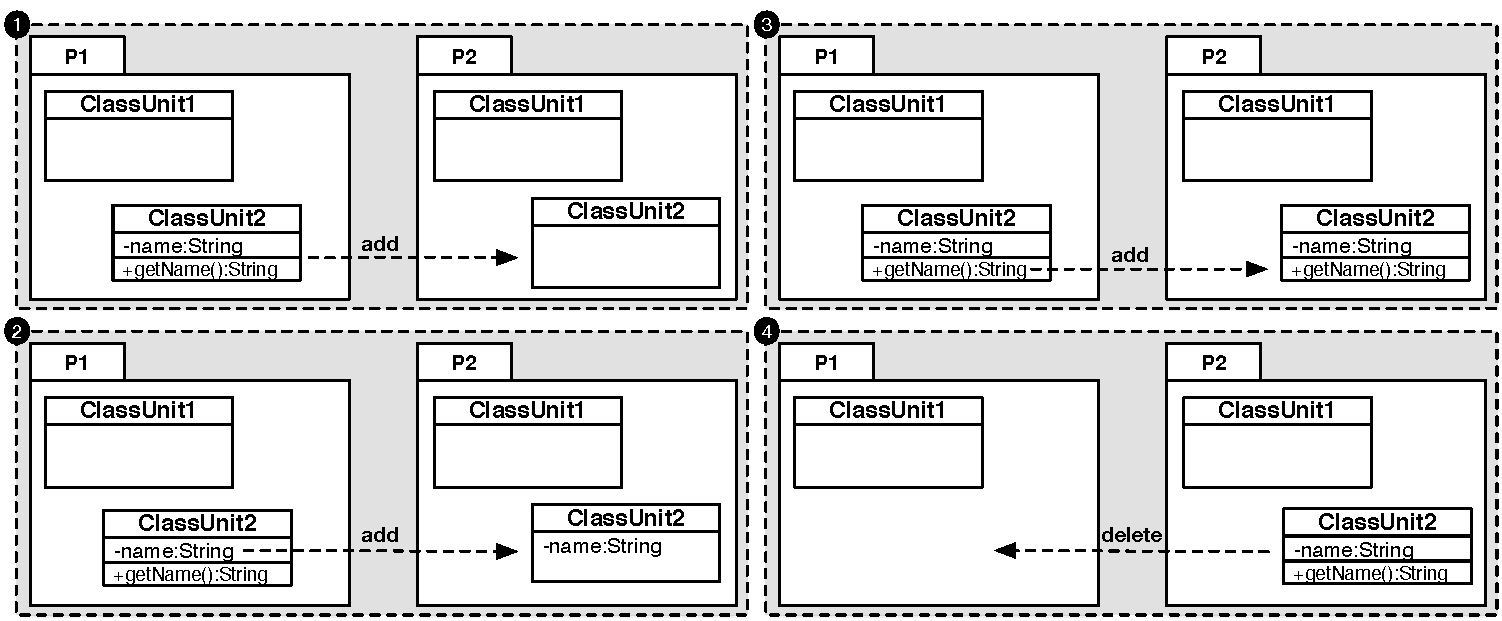
\includegraphics[scale=0.63]{images/moveNested}
	\fautor
\end{figure}

\begin{algoritmo}[!h]
     \SetAlgoLined
     \KwIn{(M, N) onde \textit{M} é uma instância da metaclasse do KDM a ser movida, \textit{N} é uma instância da metaclasse do KDM movida}
     \KwOut{Uma lista de operações primitivas (add, delete)}
     \Begin{
     \If {M instanceOf Package}{
     	\ForEach{M.codeElement()} {
     		listPrimitives.put(add)
     	}}
     \ElseIf{M instanceOf InterfaceUnit} {
     	\ForEach{M.codeElement()} {
     		listPrimitives.put(add)
     	}
     }
     \ElseIf{M instanceOf ClassUnit} {
     	\ForEach{M.codeElement()} {
     		listPrimitives.put(add)
     	}
     }
     listPrimitives.put(delete)
    
     \Return listPrimitives
	}
     \caption{Algoritmo para criar refatorações compostas.}
     \label{alg:operacoes1}
   \end{algoritmo}

As refatorações compostas consistem em uma combinação de operações atômicas. Por exemplo, considerando a refatoração \texttt{Move ClassUnit}, ela compõe-se de duas operações atômicas: \texttt{add} e \texttt{delete}. Assim, primeiro, uma nova instância da metaclasse \texttt{ClassUnit} deve ser adicionada no pacote onde se almeja mover essa instância (ver Figura~\ref{fig:operacoes_compostas_figuras}~\ding{202}). Porém, usualmente, a classe a ser movida contém atributos e/ou métodos (\texttt{StorableUnits} e/ou \texttt{MethodUnits}). Dessa forma, o engenheiro de modernização pode utilizar o Algoritmo~\ref{alg:operacoes1} para verificar quais operações atômicas precisam ser implementadas. Esse algoritmo verifica se as instâncias das metaclasses \texttt{Package}, \texttt{InterfaceUnit} e \texttt{ClassUnit} possuem elementos internos (hierarquia); no caso da metaclasse \texttt{Package}, pode-se haver pacotes internos e/ou classes; na instância da metaclasse \texttt{ClassUnit}, pode-se conter \texttt{ClassUnits}, \texttt{StorableUnits} e/ou \texttt{MethodUnits}; e na instância da metaclasse \texttt{InterfaceUnit}, pode-se haver também \texttt{StorableUnits} e/ou \texttt{MethodUnits}. 

Por exemplo, ainda considerando os exemplos ilustrados na Figura~\ref{fig:operacoes_compostas_figuras}, é possível notar que a instância da metaclasse \texttt{ClassUnit} a ser movida possui atributos e/ou métodos (\texttt{StorableUnits} e/ou \texttt{MethodUnits}), então, tais atributos e/ou métodos, também devem ser movidos (\texttt{add} e \texttt{delete}) (ver Algoritmo~\ref{alg:operacoes1}). Na Figura~\ref{fig:operacoes_compostas_figuras}~\ding{203}, uma instância da metaclasse \texttt{StorableUnit} denominada \texttt{name}, é criada e adicionada na instância da metaclasse \texttt{ClassUnit}, a qual foi criada na Figura~\ref{fig:operacoes_compostas_figuras}~\ding{202}. Similarmente, uma instância da metaclasse \texttt{MethodUnit} denominada \texttt{getName()}, também é criada e adicionada na instância da metaclasse \texttt{ClassUnit} (ver Figura~\ref{fig:operacoes_compostas_figuras}~\ding{204}). Caso a instância da \texttt{ClassUnit} que se almeja mover possua \textit{n} elementos, então, esse processo deve-se repetir \textit{n} vezes (ver Algoritmo~\ref{alg:operacoes1}). Após adicionar todos os atributos e/ou métodos na instância da \texttt{ClassUnit}, a instância da metaclasse \texttt{ClassUnit} contida no pacote \aspas{P1} pode ser removida e, assim, seus atributos e/ou métodos também são deletados.


%deve-se aplicar a operação atômica \texttt{delete} na instância da metaclasse \texttt{ClassUnit} antiga. 

%Similarmente, 
Por meio da junção dessas operações atômicas, é possível criar refatorações já existentes na literatura para o KDM. Por exemplo, podem-se focar as refatorações propostas por~\citeonline{Fowler1999}, as quais podem ser facilmente criadas para o KDM. Na Tabela~\ref{tab:refatoringsCatalogo}, algumas refatorações propostas por~\citeonline{Fowler1999} são apresentadas ressaltando a classificação da refatoração e qual(is) a(s) operação(ões) deve(m) ser utilizada(s) para criar a refatoração. A última coluna da Tabela~\ref{tab:refatoringsCatalogo} apenas ilustra as operações atômicas que serão utilizadas e não a quantidade de operações atômicas para efetivamente criar a refatoração. Nota-se que as refatorações apresentadas nessa tabela seguem a mesma convenção de nomenclatura definida por~\citeonline{Fowler1999}. Porém, os nomes de algumas refatorações foram alterados para indicar o metamodelo KDM como seu novo domínio de aplicação, por exemplo, \texttt{MoveMethod} torna-se \texttt{MoveMethodUnit} e \texttt{MoveAttribute} torna-se \texttt{MoveStorableUnit}, etc.


%Na Tabela~\ref{tab:refatoringsCatalogo} as refatorações que podem ser facilmente criadas para o metamodelo KDM são apresentadas.

\begin{table}[h]
\caption{Refatorações criadas para o metamodelo KDM.\label{tab:refatoringsCatalogo}}
\begin{center}
\begin{tabular}{ | m{4.5cm} | m{2.5cm} | m{4cm}| } 
\hline
\multicolumn{1}{|c|}{Refatoração} & \multicolumn{1}{|c|}{Classificação} & \multicolumn{1}{|c|}{Tipo de Operação}\\ 
\hline
\multicolumn{1}{|c|}{\textit{Add Package}} &  \multicolumn{1}{c|}{Atômica} & \multicolumn{1}{c|}{\texttt{add}}\\ 
\hline
\multicolumn{1}{|c|}{\textit{Add ClassUnit}} &  \multicolumn{1}{c|}{Atômica} & \multicolumn{1}{c|}{\texttt{add}}\\ 
\hline
\multicolumn{1}{|c|}{\textit{Add StorableUnit}} &  \multicolumn{1}{c|}{Atômica} & \multicolumn{1}{c|}{\texttt{add}}\\ 
\hline
\multicolumn{1}{|c|}{\textit{Add MethodUnit}} &  \multicolumn{1}{c|}{Atômica} & \multicolumn{1}{c|}{\texttt{add}}\\ 
\hline
\multicolumn{1}{|c|}{\textit{Delete Package}} &  \multicolumn{1}{c|}{Atômica} & \multicolumn{1}{c|}{\texttt{delete}}\\ 
\hline
\multicolumn{1}{|c|}{\textit{Delete ClassUnit}} &  \multicolumn{1}{c|}{Atômica} & \multicolumn{1}{c|}{\texttt{delete}}\\ 
\hline
\multicolumn{1}{|c|}{\textit{Delete StorableUnit}} &  \multicolumn{1}{c|}{Atômica} & \multicolumn{1}{c|}{\texttt{delete}}\\ 
\hline
\multicolumn{1}{|c|}{\textit{Delete MethodUnit}} &  \multicolumn{1}{c|}{Atômica} & \multicolumn{1}{c|}{\texttt{delete}}\\ 
\hline
\multicolumn{1}{|c|}{\textit{Rename Package}} &  \multicolumn{1}{c|}{Atômica} & \multicolumn{1}{c|}{\texttt{change}}\\ 
\hline
\multicolumn{1}{|c|}{\textit{Rename ClassUnit}} &  \multicolumn{1}{c|}{Atômica} & \multicolumn{1}{c|}{\texttt{change}}\\ 
\hline
\multicolumn{1}{|c|}{\textit{Rename StorableUnit}} & \multicolumn{1}{c|}{Atômica} & \multicolumn{1}{c|}{\texttt{change}}\\ 
\hline
\multicolumn{1}{|c|}{\textit{Rename MethodUnit}} &  \multicolumn{1}{c|}{Atômica} & \multicolumn{1}{c|}{\texttt{change}}\\ 
\hline
\multicolumn{1}{|c|}{\textit{Move StorableUnit}} &  \multicolumn{1}{c|}{Composta} & \multicolumn{1}{c|}{\texttt{add} $|$ \texttt{delete}}\\ 
\hline
\multicolumn{1}{|c|}{\textit{Move MethodUnit}} &  \multicolumn{1}{c|}{Composta} & \multicolumn{1}{c|}{\texttt{add} $|$ \texttt{delete}}\\ 
\hline
\multicolumn{1}{|c|}{\textit{Extract ClassUnit}} &  \multicolumn{1}{c|}{Composta} & \multicolumn{1}{c|}{\texttt{add} $|$ \texttt{delete} $|$ \texttt{change}}\\
\hline
\multicolumn{1}{|c|}{\textit{Inline ClassUnit}} &  \multicolumn{1}{c|}{Composta} & \multicolumn{1}{c|}{\texttt{change} $|$ \texttt{delete}}\\ 
\hline
\multicolumn{1}{|c|}{\textit{Flatten Hierarchy}} &  \multicolumn{1}{c|}{Composta} & \multicolumn{1}{c|}{\texttt{add} $|$ \texttt{delete} $|$ \texttt{change}}\\ 
\hline
\multicolumn{1}{|c|}{\textit{Push Down MethodUnit}} &  \multicolumn{1}{c|}{Composta} & \multicolumn{1}{c|}{\texttt{add} $|$ \texttt{delete}}\\ 
\hline
\multicolumn{1}{|c|}{\textit{Push Down StorableUnit}} &  \multicolumn{1}{c|}{Composta} & \multicolumn{1}{c|}{\texttt{add} $|$ \texttt{delete}}\\ 
\hline
\multicolumn{1}{|c|}{\textit{Pull Up MethodUnit}} &  \multicolumn{1}{c|}{Composta} & \multicolumn{1}{c|}{\texttt{add} $|$ \texttt{delete}}\\
\hline
\multicolumn{1}{|c|}{\textit{Pull Up StorableUnit}} &  \multicolumn{1}{c|}{Composta} & \multicolumn{1}{c|}{\texttt{add} $|$ \texttt{delete}}\\
\hline
\multicolumn{1}{|c|}{\textit{Extract SubClass}} &  \multicolumn{1}{c|}{Composta} & \multicolumn{1}{c|}{\texttt{add} $|$ \texttt{change}}\\
\hline
\multicolumn{1}{|c|}{\textit{Encapsulate StorableUnit}} &  \multicolumn{1}{c|}{Composta} & \multicolumn{1}{c|}{\texttt{add} $|$ \texttt{change}}\\
\hline
\end{tabular}
\end{center}
\end{table}

Após o engenheiro de modernização escolher qual refatoração irá criar para o metamodelo KDM e identificar qual(is) é(são) a(s) operação(ões) que compõe(m) a refatoração escolhida, o próximo passo é a implementação da refatoração utilizando técnicas e linguagem de transformação em modelo.

\subsection{Implementar Operações}\label{sec:linguagemDeTransformacaoUtilizada}

%Neste passo, o objetivo é implementar as operações identificadas no passo anterior. Os artefatos de entrada para a correta condução deste passo são: (\textit{i}) linguagens 

%identificar as metaclasses do KDM que serão usadas na refatoração que será implementada para o KDM. Os artefatos de entrada para a correta condução deste passo são: (\textit{i}) Mapeamento KDM - POO e (\textit{ii}) Refatoração Desejada. Após a conclusão deste passo, o artefato gerado é uma lista contendo todas as metaclasses que serão utilizadas na criação da refatoração para o KDM.


Neste passo, o engenheiro de modernização deve implementar as operações atômicas. Os artefatos de entrada para a correta condução deste passo são: (\textit{i}) linguagem de transformação e (\textit{ii}) um conjunto de \textit{templates}. Após a condução deste passo, o artefato gerado é uma lista de operações atômicas implementadas em ATL. 

%Na literatura, é possível identificar um conjunto de técnicas e linguagens específicas para auxiliar a condução e especificação de transformação de modelos~\cite{Biehl_2010, Mens_2006, Allilaire_06}. As duas abordagens mais utilizadas na literatura para a elaboração e condução de transformações/refatoração de modelos são: (\textit{i}) abordagem de manipulação direta e (\textit{ii}) abordagem de transformação genérica. A primeira utiliza linguagens de programação tradicional para a aplicação das refatorações. Ferramentas que utilizam essa abordagem usam linguagens como Java, C, C++ etc.~\cite{Bruneliere_2014}. Usualmente, tais linguagens proporcionam uma infraestrutura mínima para organizar as transformações. Algumas características de suma importância para refatorações de modelo, como regras de transformações e preservação de comportamento, são usualmente criadas pelo engenheiro, uma vez que tais linguagens não possuem API para lidar com tais características. Dessa forma, refatorações que utilizam essa abordagem tornam-se dependentes de plataformas, afetando a reusabilidade das refatorações. A segunda abordagem, transformação genérica, utiliza linguagens desenvolvidas especialmente para realizar transformações em modelos, tais como ATL, QVT, Kermeta, etc. Usualmente, tais abordagens são conhecidas como endógenas e são implementadas utilizando técnicas de reescrita de grafo (ver Capítulo~\ref{chapter:fundamentacao_teorica} Seção~\ref{sec:transformacoes_de_modelos}). Diferentemente da primeira abordagem, a segunda abordagem facilita o reúso de refatorações. Por exemplo, utilizando a segunda abordagem, o engenheiro de modernização pode criar um conjunto de regras de refatorações por meio de linguagens de transformações genéricas, podendo tais refatorações serem invocadas, utilizando qualquer linguagem de programação. O engenheiro de modernização pode escrever um código em Java que tem como entrada uma instância do metamodelo KDM para ser refatorado, a reforação a ser aplicada nessa instância e um conjunto de parâmetros para realizar a refatoração na instância do metamodelo KDM.

%Dada essa motivação, no presente trabalho, a segunda abordagem é utilizada. Mais especificamente, a linguagem de transformação ATL~\cite{ATL_eclipse,Jouault_2008} foi escolhida para definir e implementar refatorações em instâncias do metamodelo KDM. ATL foi escolhida como linguagem de transformação considerando vários aspectos. Essa linguagem está integrada no ambiente de desenvolvimento Eclipse, o que fornece uma série de recursos padrões para o desenvolvimento (\textit{syntax highlighting} e \textit{debugger}). Além disso, ATL é parte do projeto \textit{Model-To-Model} e possui um grupo\footnote{\texttt{http://www.eclipse.org/forums/}} de discussão ativo, constantemente atualizado, vários exemplos e diversos estudos de casos aplicados até mesmo na indústria utilizam essa linguagem.


%ATL possui um módulo de execução denominado \textit{refining}, que é utilizado para criar refatorações em nível de modelo. Esse módulo foi introduzido para facilitar a programação de refatorações. Com o módulo \textit{refining}, os engenheiros de modernização podem se concentrar no código ATL, dedicado à geração de elementos estruturados modificados. Outros elementos estruturados do KDM (por exemplo, aqueles que permanecem inalteradas antes e após a refatoração) são implicitamente processados pelo mecanismo da ATL. O módulo \textit{refining} pode ser utilizado simplesmente substituindo a palavra-chave \texttt{from} pela \texttt{refining}. Obviamente, o modo de \textit{refining} só pode ser utilizado para as transformações endógenas (\aspas{\textit{in-place}}) (ver Capítulo~\ref{chapter:fundamentacao_teorica}, Seção~\ref{sec:transformacoes_de_modelos})


Como apresentado na Seção~\ref{sec:refatoracao_para_o_metamodelo_kdm}, as refatorações no contexto desta tese são agrupadas em dois níveis de operações: (\textit{i}) operações atômicas e (\textit{ii}) operações compostas. As granularidades definidas como operações atômicas são: \texttt{add}, \texttt{delete} e \texttt{change}. Essas operações atômicas podem ser facilmente implementadas em ATL. Dessa forma, um \textit{template} para cada operação atômica é disponibilizado como artefato para auxiliar o engenheiro de modernização a criar refatorações para o KDM. O \textit{template} para a operação atômica \texttt{add} é apresentado no Código-fonte~\ref{codigo:template_addKDMElement}. As partes fixas dos \textit{templates} são formadas por texto ATL e as partes variantes são formadas por três tipos de instruções: (\textit{i}) argumentos, \textbf{ArgX}\footnote{\textbf{ArgX}, onde \textbf{X} representa um número sequencial dos argumentos. \label{foot:Arg}}, demarcados pelos símbolos \aspas{\textbf{<\#}} e \aspas{\textbf{\#>}} e que devem ser substituídos por \textit{strings} válidas na linguagem ATL; (\textit{ii}) argumentos, \textbf{ArgX}\textsuperscript{\ref{foot:Arg}}, demarcados pelos símbolos \aspas{\textbf{<\%}} e \aspas{\textbf{\%>}} e que devem ser substituídos por metaclasses do metamodelo KDM, por exemplo, \texttt{ClassUnit}, \texttt{InterfaceUnit}, \texttt{StorableUnit}, \texttt{MethodUnit}, etc; (\textit{iii}) argumentos, \textbf{ArgX}\textsuperscript{\ref{foot:Arg}}, demarcados pelos símbolos \aspas{\textbf{<$@$}} e \aspas{\textbf{@>}}, que devem ser substituídos de acordo com o domínio do sistema que será aplicada a refatoração, por exemplo, nomes de pacotes, classes, interfaces, atributos, métodos, etc.  

%argumentos, \textbf{ArgX} onde X representa um número cardinal, demarcadas pelos símbolos \aspas{\textbf{<\%}} e \aspas{\textbf{\%>}} ou \aspas{\textbf{<$@$}} e \aspas{\textbf{@>}}. O primeiro símbolo (\aspas{\textbf{<\%}} e \aspas{\textbf{\%>}}) informa para o engenheiro de modernização que metaclasses do KDM devem ser substituídas pelo argumento.

%Deve-se também utilizar outro artefato para auxiliar o engenheiro de modernização a substituir as partes variáveis do \textit{template} de forma correta.

%Outro artefato que deve ser utilizado juntamente com o \textit{template} apresentado no Código-fonte~\ref{codigo:template_addKDMElement} para auxiliar o engenheiro de modernização a criar a operação atômica é a Tabela X. Essa tabela é utilizada como um guia para conduzir o engenheiro de modernização a especificar corretamente os as partes variantes do \textit{template}, ou seja, os argumentos.





\begin{codigo}[caption={[\textit{Template} ATL para realizar a operação atômica \texttt{add}.] \textit{Template} ATL para realizar a operação atômica \texttt{add}.},escapeinside={(*@}{@*)}, basicstyle=\footnotesize, label={codigo:template_addKDMElement}, language=ATL]{Name}
rule create(*@<\textbf{\#Arg1\#}>@*){
	from
		source : MM!(*@<\textbf{\%Arg2\%}>@*) (source.name = (*@<\textbf{$@$Arg3@}>@*))
	to 
		target: MM!(*@<\textbf{\%Arg2\%}>@*) (
			codeElement (*@$\leftarrow$@*) source.codeElement(*@$\rightarrow$@*)including(newElement)
		),
		newElement: MM!(*@<\textbf{\%Arg4\%}>@*) (
			name (*@$\leftarrow$@*) (*@<\textbf{$@$Arg5@}>@*)
		)
}
\end{codigo}


%para adicionar uma nova instância da metaclasse \texttt{ClassUnit} denominada \texttt{\aspas{novaClassUnit}} no pacote \texttt{com.br.teste}. Como pode ser observado na linha 5 é especificado o nome do pacote (\texttt{\aspas{com.br.teste}}) que é onde a nova instância da \texttt{ClassUnit} será adicionada. A linha 8 representa que a nova instância da \texttt{ClassUnit} será adicionada no associação \texttt{codeElement}. Nas linhas 10-12 uma nova instância da metaclasse \texttt{ClassUnit} é adicionada e seu nome definido como \aspas{novaClassUnit}.

%Mostrar que o Engenheiro de modernização pode adaptar qualquer elemento... Mostrar uma exemplo em ATL onde pode ser substituido pela metaclasse do KDM........

Além do \textit{template} apresentado no Código-fonte~\ref{codigo:template_addKDMElement}, outro artefato também deve ser utilizado para auxiliar o engenheiro de modernização a substituir as partes variáveis do \textit{template} de forma correta. Esse artefato é apresentado na Tabela~\ref{tab:guia_template_operacao_add}, o qual é utilizado como um guia para conduzir o engenheiro de modernização a especificar corretamente as partes variantes do \textit{template}, ou seja, os argumentos.

\begin{table}[h]
\centering
\caption{Guia para auxiliar a substituição dos argumentos do \textit{template} apresentado no Código-fonte~\ref{codigo:template_addKDMElement}.}
\label{tab:guia_template_operacao_add}
\begin{tabular}{ | m{1.7cm} | m{12cm}| } 
\hline
\multicolumn{1}{|c|}{Argumentos}                                         & \multicolumn{1}{c|}{Valores} \\ \hline
%\multicolumn{1}{|c|}{\textbf{<\#Arg1\#>}} & Nome do módulo. Pode-se utilizar qualquer \textit{string} válida na linguagem ATL. \\ 
%\hline
\multicolumn{1}{|c|}{\textbf{<\#Arg1\#>}} & Nome da regra. Pode-se utilizar qualquer \textit{string} válida na linguagem ATL. \\  
\hline
\multicolumn{1}{|c|}{\textbf{<\%Arg2\%>}} & Nome de uma metaclasse (\texttt{ClassUnit}, \texttt{InterfaceUnit}, \texttt{StorableUnit}, \texttt{MethodUnit}, etc). Deve-se especificar o nome da metaclasse que conterá a nova instância da metaclasse a ser criada. \\ 
\hline
\multicolumn{1}{|c|}{\textbf{<$@$Arg3@>}} & Nome da instância do elemento estrutural especificado no \textbf{<\%Arg2\%>}. Deve-se especificar o nome da instância da metaclasse que conterá a nova instância da metaclasse a ser criada. Esse argumento depende do domínio do sistema que será aplicada a refatoração e é identificada no meta-atributo \texttt{name} das metaclasses do KDM.  \\ 
\hline
\multicolumn{1}{|c|}{\textbf{<\%Arg4\%>}} & Nome de uma metaclasse que será instanciada. Deve-se especificar o nome da metaclasse que será criada.  \\ 
\hline
\multicolumn{1}{|c|}{\textbf{<$@$Arg5@>}} & Nome da nova instância que será criada. Deve-se especificar o nome da instância da metaclasse que será criada. Esse argumento também depende do domínio do sistema que será aplicado à refatoração.  \\ 
\hline
\end{tabular}
\end{table}

Dado o \textit{template} apresentado no Código-fonte~\ref{codigo:template_addKDMElement}, bem como as Tabelas~\ref{tab:mapemanetoEntreOOPeKDM} e~\ref{tab:guia_template_operacao_add}, a combinação desses três artefatos auxiliam/guiam o engenheiro de modernização a criar a operação atômica \texttt{add} para um determinado elemento estrutural do KDM, ou seja, \texttt{ClassUnit}, \texttt{InterfaceUnit}, \texttt{Package}, \texttt{StorableUnit}, \texttt{MethodUnit}, etc. Por exemplo, 
%
%
%quando combinado com a Tabela~\ref{x} (os elementos estruturais \texttt{ClassUnit}, \texttt{InterfaceUnit}, \texttt{Package}, \texttt{StorableUnit}, \texttt{MethodUnit}, etc) e Tabela X auxiliam a originar a operação atômica \texttt{add} para um determinado elemento estrutural do KDM. 
%
%
%os elemennnnnntos estruturais (\texttt{ClassUnit}, \texttt{InterfaceUnit}, \texttt{Package}, \texttt{StorableUnit}, \texttt{MethodUnit}, etc) apresentado na Tabela~\ref{tab:mapemanetoEntreOOPeKDM} origina uma operação atômica \texttt{add} para um determinado elemento estrutu
%
no Código-fonte~\ref{codigo:exemplo_add_classUnit} é apresentada uma simples ATL que foi criada utilizando esses três artefatos. O argumento \textbf{<\#Arg1\#>} foi substituído pela \textit{string} \texttt{Class}, respectivamente, ver linha 1. Na linha 3, \textbf{<\%Arg2\%>} foi substituído pela metaclasse \texttt{Package} e o argumento \textbf{<$@$Arg3$@$>} foi substituído pela \textit{String} \texttt{\aspas{com.br.teste}}, a qual representa o nome da instância da metaclasse \texttt{Package} onde uma nova instância da metaclasse \texttt{ClassUnit} será adicionada. Finalmente, os argumentos \textbf{<\%Arg4\%>} e \textbf{<$@$Arg5$@$>} foram substituídos pela metaclasse \texttt{ClassUnit} e pela \textit{String} \texttt{\aspas{novaClassUnit}}, ver linhas 8 e 9.  A execução desse código cria uma nova instância da metaclasse \texttt{ClassUnit} denominada \aspas{novaClassUnit} no pacote \aspas{com.br.teste}.

\begin{codigo}[caption={[ATL para realizar a operação atômica \texttt{add} \texttt{ClassUnit}.] ATL para realizar a operação atômica \texttt{add} \texttt{ClassUnit}.},escapeinside={(*@}{@*)}, basicstyle=\footnotesize, label={codigo:exemplo_add_classUnit}, language=ATL]{Name}
rule createClass{
	from
		source : MM!Package (source.name = (*@\aspas{com.br.teste}@*))
	to 
		target: MM!Package (
			codeElement (*@$\leftarrow$@*) source.codeElement(*@$\rightarrow$@*)including(newElement)
		),
		newElement: MM!ClassUnit (
			name (*@$\leftarrow$@*) (*@\aspas{novaClassUnit}@*)
		)
}
\end{codigo}


Similarmente, o engenheiro de modernização pode implementar a operação atômica \texttt{delete} facilmente seguindo um \textit{template}. O \textit{template} responsável pela operação atômica \texttt{delete} é apresentado no Código-fonte~\ref{codigo:template_delete}\footnote{A palavra-chave \texttt{drop} é utilizada na linha 5 do Código-fonte~\ref{codigo:template_delete} para especificar que uma determinada instância será removida.}. Esse \textit{template} também possui partes fixas e partes variantes. As partes fixas são textos em ATL e as partes variantes são formadas por argumentos demarcados pelas instruções \aspas{\textbf{<\#}} e \aspas{\textbf{\#>}}, \aspas{\textbf{<\%}} e \aspas{\textbf{\%>}} e \aspas{\textbf{<$@$}} e \aspas{\textbf{$@$>}}. 

O guia para auxiliar o engenheiro de modernização a especificar corretamente as partes variantes do \textit{template} \texttt{delete} é apresentado na Tabela~\ref{tab:guia_template_operacao_delete}. Por meio de três artefatos: (\textit{i}) o \textit{template} representado no Código-fonte~\ref{codigo:template_delete}, (\textit{ii}) o mapeamento entre OO e KDM apresentado na Tabela~\ref{tab:mapemanetoEntreOOPeKDM}, (\textit{iii}) e o guia apresentado na Tabela ~\ref{tab:guia_template_operacao_delete}, o engenheiro de modernização pode criar a operação atômica \texttt{delete}. Por exemplo, pode-se considerar Código-fonte~\ref{codigo:exemplo_delete_classUnit}, onde almeja-se remover uma instância da metaclasse \texttt{ClassUnit}. 

\begin{codigo}[caption={[\textit{Template} ATL para realizar a operação atômica \texttt{delete}.] \textit{Template} ATL para realizar a operação atômica \texttt{delete}.},escapeinside={(*@}{@*)}, basicstyle=\footnotesize, label={codigo:template_delete}, language=ATL]{Name}
rule delete(*@<\textbf{\#Arg1\#}>@*) {
  from
      source : MM!(*@<\textbf{\%Arg2\%}>@*) (source.name = (*@<\textbf{$@$Arg3$@$}>@*) and source.refImmediateComposite().name = (*@<\textbf{$@$Arg4$@$}>@*)
  to
      drop
}
\end{codigo}

\begin{table}[h]
\centering
\caption{Guia para auxiliar a substituição dos argumentos do \textit{template} apresentado no Código-fonte~\ref{codigo:template_delete}.}
\label{tab:guia_template_operacao_delete}
\begin{tabular}{ | m{1.7cm} | m{12cm}| } 
\hline
\multicolumn{1}{|c|}{Argumentos}                                         & \multicolumn{1}{c|}{Valores} \\ \hline
%\multicolumn{1}{|c|}{\textbf{<\#Arg1\#>}} & Nome do módulo. Pode-se utilizar qualquer \textit{string} válida na linguagem ATL. \\ 
%\hline
\multicolumn{1}{|c|}{\textbf{<\#Arg1\#>}} & Nome da regra. Pode-se utilizar qualquer \textit{string} válida na linguagem ATL. \\  
\hline
\multicolumn{1}{|c|}{\textbf{<\%Arg2\%>}} & Nome de uma metaclasse (\texttt{ClassUnit}, \texttt{InterfaceUnit}, \texttt{StorableUnit}, \texttt{MethodUnit}, etc). Deve-se especificar o nome da metaclasse que representa a instância da metaclasse a ser deletada. \\ 
\hline
\multicolumn{1}{|c|}{\textbf{<$@$Arg3@>}} & Nome da instância do elemento estrutural especificado no \textbf{<\%Arg2\%>}. Deve-se especificar o nome da instância da metaclasse que representa a instância da metaclasse a ser deletada. Esse argumento depende do domínio do sistema que será aplicada à refatoração e é identificada no meta-atributo \texttt{name} das metaclasses do KDM.  \\ 
\hline
\multicolumn{1}{|c|}{\textbf{<$@$Arg4@>}} & Nome da instância do elemento estrutural que contém o elemento especificado no \textbf{<\%Arg2\%>}. Deve-se especificar o nome da instância da metaclasse que possui a instância da metaclasse a ser deletada. Esse argumento depende do domínio do sistema que será aplicada à refatoração e é identificada no meta-atributo \texttt{name} das metaclasses do KDM.  \\ 
\hline
\end{tabular}
\end{table}

\begin{codigo}[caption={[ATL para realizar a operação atômica \texttt{delete} \texttt{ClassUnit}.] ATL para realizar a operação atômica \texttt{delete} \texttt{ClassUnit}.},escapeinside={(*@}{@*)}, basicstyle=\footnotesize, label={codigo:exemplo_delete_classUnit}, language=ATL]{Name}
rule deleteClass {
  from
      source : MM!ClassUnit (source.name = (*@\aspas{ClassToRemove}@*) and source.refImmediateComposite().name = (*@\aspas{PackageThatContainsTheClassToRemove}@*))
  to
      drop
}
\end{codigo}

O argumento \textbf{<\#Arg1\#>} foi substituído pela \textit{String} \texttt{Class} (ver linha 1). Depois, na linha 3 o argumento \textbf{<\%Arg2\%>} foi substituído pela metaclasse \texttt{ClassUnit} e o argumento \textbf{<$@$Arg3$@$>} foi substituído pela \textit{String} \texttt{\aspas{ClassToRemove}}. Essa \textit{String} representa o nome da instância da \texttt{ClassUnit} que se almeja deletar. O argumento \textbf{<$@$Arg4$@$>} foi substituído pela \textit{String}\texttt{\aspas{Package\-ThatContainsTheClassToRemove}}, a qual representa o pacote que contém a classe que será deletada.


Finalmente, a operação atômica \texttt{change} também pode ser implementada por meio de \textit{template}. O Código-fonte~\ref{codigo:template_change} representa o \textit{template} da operação atômica \texttt{change}. Esse \textit{template} também possui partes fixas e instruções demarcadas por \aspas{\textbf{<\#}} e \aspas{\textbf{\#>}}, \aspas{\textbf{<\%}} e \aspas{\textbf{\%>}} e \aspas{\textbf{<$@$}} e \aspas{\textbf{$@$>}} que representam as partes variantes.

\begin{codigo}[caption={[\textit{Template} para realizar a operação atômica \texttt{change}.] \textit{Template} para realizar a operação atômica \texttt{change}.},escapeinside={(*@}{@*)}, basicstyle=\footnotesize, label={codigo:template_change}, language=ATL]{Name}
rule change(*@<\textbf{\#Arg1\#}>@*) {
	from
		source : MM!(*@<\textbf{\%Arg2\%}>@*) (source.name=(*@<\textbf{$@$Arg3$@$}>@*))
	to 
		target : MM!(*@<\textbf{\%Arg2\%}>@*) (
			(*@<\textbf{\%Arg4\%}>@*) (*@$\leftarrow$@*) (*@<\textbf{$@$Arg5$@$}>@*)
		)
}
\end{codigo}

\begin{table}[h]
\centering
\caption{Guia para auxiliar a substituição dos argumentos do \textit{template} apresentado no Código-fonte~\ref{codigo:template_change}.}
\label{tab:guia_template_operacao_change}
\begin{tabular}{ | m{1.7cm} | m{12cm}| } 
\hline
\multicolumn{1}{|c|}{Argumentos}                                         & \multicolumn{1}{c|}{Valores} \\ \hline
%\multicolumn{1}{|c|}{\textbf{<\#Arg1\#>}} & Nome do módulo. Pode-se utilizar qualquer \textit{string} válida na linguagem ATL. \\ 
%\hline
\multicolumn{1}{|c|}{\textbf{<\#Arg1\#>}} & Nome da regra. Pode-se utilizar qualquer \textit{string} válida na linguagem ATL. \\  
\hline
\multicolumn{1}{|c|}{\textbf{<\%Arg2\%>}} & Nome de uma metaclasse (\texttt{ClassUnit}, \texttt{InterfaceUnit}, \texttt{StorableUnit}, \texttt{MethodUnit}, etc). Deve-se especificar o nome da metaclasse que conterá a instância da metaclasse a ser alterada. \\ 
\hline
\multicolumn{1}{|c|}{\textbf{<$@$Arg3@>}} & Nome da instância do elemento estrutural especificado no \textbf{<\%Arg2\%>}. Deve-se especificar o nome da instância da metaclasse a ser alterada. Esse argumento depende do domínio do sistema que será aplicada à refatoração e é identificada no meta-atributo \texttt{name} das metaclasses do KDM.  \\ 
\hline
\multicolumn{1}{|c|}{\textbf{<\%Arg4\%>}} & Nome do(s) meta-atributo(s) da metaclasse que será alterada. Deve-se especificar o(s) nome(s) do(s) meta-atributo(s) que será(ão) alterado(s).  \\ 
\hline
\multicolumn{1}{|c|}{\textbf{<$@$Arg5$@$>}} & Novo(s) valor(es) para ser setado(s) no(s) meta-atributo(s) especificado(s) no \textbf{<\%Arg4\%>}. Esse argumento também depende do domínio do sistema que será aplicada à refatoração.  \\ 
\hline
\end{tabular}
\end{table}

Na Tabela~\ref{tab:guia_template_operacao_change}, o guia para auxiliar o engenheiro de modernização a especificar corretamente as partes variantes do \textit{template} \texttt{change} é apresentado. A junção dos três artefatos: (\textit{i}) o \textit{template} apresentado no Código-fonte~\ref{codigo:template_change}, (\textit{ii}) o mapemanto entre OO e KDM (ver Tabela~\ref{tab:mapemanetoEntreOOPeKDM}) e (\textit{iii}) o guia apresentado na Tabela~\ref{tab:guia_template_operacao_change} auxilia o engenheiro de modernização a criar a operação atômica \texttt{change}. Por exemplo, pode-se considerar o Código-fonte~\ref{codigo:exemplo_rename_Package} onde esses três artefatos foram utilizados pelo engenheiro de modernização para implementar a operação atômica \texttt{change}. Nesse código-fonte, uma determinada instância da metaclasse \texttt{Package} é alterada, ou seja, seu meta-atributo \texttt{name} é renomeado. Assim, o argumento \textbf{<\#Arg1\#>} foi substituído pela \textit{string} \texttt{Package} (linha 1). Na linha 3 \textbf{<\%Arg2\%>} foi substituído pela metaclasse \texttt{Package} e o argumento \textbf{<$@$Arg3$@$>} foi substituído pela \textit{String} \texttt{\aspas{PackageToRename}}, a qual representa o nome da instância da metaclasse \texttt{Package} onde uma nova instância da metaclasse \texttt{ClassUnit} será alterada. O argumento \textbf{<\%Arg4\%>} foi substituído pelo meta-atributo \texttt{name} e o \textbf{<$@$Arg5$@$>} foi substituído por uma \textit{String} que representa o novo nome da instância da metaclasse \texttt{Package} (ver linha 6).


%A última operação atômica é a operação \texttt{change}. Essa operação é responsável por alterar o valor de um meta-atributo de uma metaclasse do metamodelo KDM, como por exemplo \textit{Rename Package} apresentado no Código-fonte~\ref{codigo:exemplo_rename_Package}. Na linha 5 é especificado e identificado a instância da metaclasse \texttt{Package} que será alterada. Nas linhas 7-9 a instância especificada da metaclasse \texttt{Package} é alterada.

\begin{codigo}[caption={[ATL para realizar a operação atômica \texttt{change} \texttt{ClassUnit}.] ATL para realizar a operação atômica \texttt{change} \texttt{ClassUnit}.},escapeinside={(*@}{@*)}, basicstyle=\footnotesize, label={codigo:exemplo_rename_Package}, language=ATL]{Name}
rule changePackage {
	from
		source : MM!Package (source.name=(*@\aspas{PackageToRename}@*))
	to 
		target : MM!Package (
			name (*@$\leftarrow$@*) (*@\aspas{newName}@*)
		)
}
\end{codigo}


\subsection{Agrupar Operações}

Neste passo, o engenheiro de modernização deve agrupar as operações atômicas criadas no passo anterior para formar a refatoração para o KDM. Os artefatos de entrada para a correta execução deste passo são: (\textit{i}) as operações atômicas implementadas e (\textit{ii}) um \textit{template} para guiar o engenheiro a agrupar as operações atômicas e formar a refatoração. Após a conclusão deste passo, o artefato gerado é uma refatoração escrita em ATL para o KDM.

Como apresentado na Tabela~\ref{tab:refatoringsCatalogo}, com a combinação dessas operações atômicas os engenheiros de modernização podem criar refatorações mais significativas. Por exemplo, o Código-fonte~\ref{codigo:exemplo_add_classUnit} e o Código-fonte~\ref{codigo:exemplo_delete_classUnit} ilustram as operações atômicas \texttt{add} e \texttt{delete} para instâncias da metaclasse \texttt{ClassUnit}, respectivamente, assim, a combinação dessas duas operações atômica resulta na refatoração \texttt{move}. %Porém, engenheiros de modernização podem adaptarem esses códigos para utilizam outros elementos estruturais tais como: \texttt{InterfaceUnit}, \texttt{StorableUnit}, \texttt{MethodUnit}, etc. Por exemplo, caso almeja-se deletar uma determinada instância da metaclasse \texttt{InterfaceUnit} o engenheiro de modernização deve apenas substituir a linha 5 do Código-fonte~\ref{codigo:exemplo_delete_classUnit} por \aspas{\texttt{source: MM!InterfaceUnit(source.name = \aspas{InterfaceToRemove})}}. 

Para guiar o engenheiro de modernização a agrupar as operações atômicas e criar a refatoração, um \textit{template} deve ser utilizado. Esse \textit{template} é apresentado no Código-fonte~\ref{codigo:template_module_agrupar}, o qual contém partes fixas e instrução demarcada por \aspas{\textbf{<\#}} e \aspas{\textbf{\#>}} que que deve ser substituída por \textit{strings} válidas na linguagem ATL. Além disso, esse \textit{template} também contém trechos em pseudocódigo (\textbf{para cada}, \textbf{se}, \textbf{senão se}, etc) para auxiliar e guiar o engenheiro de modernização a agrupar corretamente as operações atômicas implementadas no passo anterior. Assim, para cada operação atômica implementada, deve-se verificar se ela é do tipo \texttt{add}, \texttt{delete} e/ou \texttt{change}. Esse processo deve ser repetido até não existir mais operações atômicas para serem copiadas ao \textit{template} apresentado no Código-fonte~\ref{codigo:template_module_agrupar}. O argumento \textbf{<\#Arg1\#>} pode ser substituido por qualquer \textit{string} válida na linguagem ATL.

\begin{codigo}[caption={[\textit{Template} ATL para agrupar as operações atômicas.] \textit{Template} ATL para agrupar as operações atômicas.},escapeinside={(*@}{@*)}, basicstyle=\footnotesize, label={codigo:template_module_agrupar}, language=ATL]{Name}
module (*@<\textbf{\#Arg1\#}>@*);
create OUT : MM refining IN : MM;
(*@ 
[\textbf{para cada} operações atômicas \textbf{faça}]@*)
    (*@[\textbf{se} operação atômica == \texttt{add} \textbf{então}]@*)
        (*@adiciona o@*) (*@\textit{template} preenchido@*) (*@do@*) (*@Código-fonte~\ref{codigo:template_addKDMElement}@*)
    (*@[\textbf{senão se} operação atômica == \texttt{delete} \textbf{então}]@*)
        (*@adiciona o@*) (*@\textit{template} preenchido@*) (*@do@*) (*@Código-fonte~\ref{codigo:template_delete}@*)
    (*@[\textbf{senão se} operação atômica == \texttt{change} \textbf{então}]@*)
        (*@adiciona o@*) (*@\textit{template} preenchido@*) (*@do@*) (*@Código-fonte~\ref{codigo:template_change}@*)
    (*@[/\textbf{fim se}]@*)
(*@[/\textbf{fim para}]@*)

\end{codigo}

Após a criação de uma refatoração, o engenheiro de modernização deve especificar as restrições da refatoração criada. Tais restrições são especificadas utilizando linguagens de restrições, por exemplo, OCL. Na próxima seção, maiores informações são apresentadas.

\subsection{Definir Restrições (Pré- e Pós-condições)}\label{sec:linguagem_de_restricao}

Neste passo, o engenheiro de modernização deve implementar as restrições (pré- e pós-condições). Os artefatos de entrada para a correta condução deste passo são: (\textit{i}) linguagem de restrição e (\textit{ii}) um conjunto de \textit{templates}. Após a condução deste passo, o artefato gerado é uma lista de restrições implementadas em OCL. 

Após o engenheiro de modernização criar uma determinada refatoração, o próximo passo consiste na criação de restrições (pré- e pós-condições) para a refatoração. Usualmente, antes e após a aplicação de uma determinada refatoração, algumas restrições precisam ser satisfeitas. Tais restrições geralmente são úteis para verificar se os parâmetros necessários para executar a refatoração foram corretamente informados, bem como verificar se a refatoração foi aplicada de forma correta. No contexto de modelos, tais restrições são especificadas utilizando linguagens como OCL e são caracterizadas como pré- e pós-condições. Além disso, essas restrições são importantes para assegurar que a refatoração será aplicada de forma correta e ainda irá preservar a semântica da instância do metamodelo. Por exemplo, verificar se uma determinada instância de uma metaclasse realmente existe antes de aplicar a operação atômica \texttt{delete}, ou verificar se uma determinada instância já existe antes de realizar a operação atômica \texttt{add}. Diante disso, cada refatoração (operação atômica) definida nesta tese está associada com uma pré- e pós-condição definida em OCL. OCL foi escolhida pois é uma linguagem padronizada pelo OMG e também possui suporte no ambiente de desenvolvimento Eclipse.

Para auxiliar o engenheiro de modernização durante a criação dessas restrições (pré- e pós-condições) \textit{templates} também foram definidos. Os \textit{templates} aqui apresentados estão associados a uma determinada operação atômica. Por exemplo, para cada operação atômica (\texttt{add}, \texttt{delete} e \texttt{change}) dois \textit{templates} foram definidos para auxiliar a criação das restrições, ou seja, um \textit{template} para auxiliar a criação da pré-condição e outro para auxiliar a criação da pós-condição.

Os \textit{templates} para a operação atômica \texttt{add} são apresentados nos Códigos-fontes~\ref{codigo:pre_template_add} e~\ref{codigo:template_pos_condicao_add}, onde o primeiro código ilustra o \textit{template} para criar a pré-condição e o segundo representa o \textit{template} para especificar a pós-condição da operação atômica \texttt{add}. As partes fixas dos \textit{templates} são formadas por texto em OCL e as partes variantes são formadas por três tipos de instruções: (\textit{i}) argumentos, \textbf{ArgX}\footnote{\textbf{ArgX}, onde \textbf{X} representa um número sequencial dos argumentos. \label{foot:Arg1}}, demarcados pelos símbolos \aspas{\textbf{<\#}} e \aspas{\textbf{\#>}} e que devem ser substituídos por \textit{strings} válidas na linguagem OCL; e (\textit{ii}) argumentos, \textbf{ArgX}\textsuperscript{\ref{foot:Arg1}}, demarcados pelos símbolos \aspas{\textbf{<\%}} e \aspas{\textbf{\%>}} e que devem ser substituídos por elementos/metaclasses do metamodelo KDM, por exemplo, \texttt{ClassUnit}, \texttt{InterfaceUnit}, \texttt{StorableUnit}, \texttt{MethodUnit}, etc; e (\textit{iii}) argumentos, \textbf{ArgX}\textsuperscript{\ref{foot:Arg}}, demarcados pelos símbolos \aspas{\textbf{<$@$}} e \aspas{\textbf{@>}} que devem ser substituídos de acordo com o domínio do sistema que será aplicado à refatoração, por exemplo, nomes de pacotes, classes, interfaces, atributos, métodos, etc.  

\begin{codigo}[caption={[\textit{Template} OCL para realizar a pré-condição da operação atômica \texttt{add}.] \textit{Template} OCL para realizar a pré-condição da operação atômica \texttt{add}.},escapeinside={(*@}{@*)}, basicstyle=\footnotesize, label={codigo:pre_template_add}, language=OCL]{Name}
context (*@<\textbf{\%Arg1\%}>@*)::(*@<\textbf{\#Arg2\#}>@*)(newName: String)
pre : (*@<\textbf{\%Arg3\%}>@*).allInstances->select(e : (*@<\textbf{\%Arg3\%}>@*) | a.name = (*@<\textbf{$@$Arg4$@$}>@*)) and not (*@<\textbf{\%Arg1\%}>@*).refImmediateComposite().codeElement(*@$\rightarrow$@*)exist (e : (*@<\textbf{\%Arg1\%}>@*) | e.name = newName)
\end{codigo}

O \textit{template} apresentado no Código-fonte~\ref{codigo:pre_template_add} tem como função verificar se uma determinada instância de uma metaclasse a ser criada pela operação atômica \texttt{add} ainda não existe na instância do KDM. Isso é importante para garantir que não existam duas instâncias iguais no KDM. Caso positivo a operação atômica pode ser executada. A pós-condição apresentada no Código-fonte~\ref{codigo:template_pos_condicao_add}, por outro lado verifica se a instância de uma metaclasse realmente foi criada pela execução da operação atômica \texttt{add}.

\begin{codigo}[caption={[\textit{Template} OCL para realizar a pós-condição da operação atômica \texttt{add}.] \textit{Template} OCL para realizar a pós-condição da operação atômica \texttt{add}.},escapeinside={(*@}{@*)}, basicstyle=\footnotesize, label={codigo:template_pos_condicao_add}, language=OCL]{Name}
context (*@<\textbf{\%Arg1\%}>@*)::(*@<\textbf{\#Arg2\#}>@*)(newName: String)
post : (*@<\textbf{\%Arg3\%}>@*).allInstances->select(e : (*@<\textbf{\%Arg3\%}>@*) | a.name = (*@<\textbf{$@$Arg4$@$}>@*)) and (*@<\textbf{\%Arg1\%}>@*).refImmediateComposite().codeElement(*@$\rightarrow$@*)exist (e : (*@<\textbf{\%Arg1\%}>@*) | e.name = newName)
\end{codigo}

\begin{table}[h]
\centering
\caption{Guia para auxiliar a substituição dos argumentos dos \textit{templates} apresentados nos Códigos-fontes~\ref{codigo:pre_template_add} e~\ref{codigo:template_pos_condicao_add}.}
\label{tab:guia_template_pre_pos_add}
\begin{tabular}{ | m{1.7cm} | m{12cm}| } 
\hline
\multicolumn{1}{|c|}{Argumentos}                                         & \multicolumn{1}{c|}{Valores} \\ \hline
\multicolumn{1}{|c|}{\textbf{<\%Arg1\%>}} & Nome de uma metaclasse (\texttt{ClassUnit}, \texttt{InterfaceUnit}, \texttt{StorableUnit}, \texttt{MethodUnit}, etc). Deve-se especificar o nome da metaclassse que foi criada pela operação atômica \texttt{add}. \\ 
\hline
\multicolumn{1}{|c|}{\textbf{<\#Arg2\#>}} & Nome da restrição. Pode-se utilizar qualquer \textit{string} válida em OCL. \\ 
\hline
\multicolumn{1}{|c|}{\textbf{<\%Arg3\%>}} & Nome de uma metaclasse que contém o elemento especificado no \textbf{<\%Arg1\%>}. Por exemplo, se o \textbf{<\%Arg1\%>} for uma \texttt{ClassUnit} e/ou \texttt{InterfaceUnit} deve-se especificar a metaclasse \texttt{Package}. \\ 
\hline
\multicolumn{1}{|c|}{\textbf{<$@$Arg4$@$>}} & Nome da instância do elemento estrutural que contém o elemento especificado no \textbf{<\%Arg3\%>}. Esse argumento depende do domínio do sistema que será aplicado à refatoração. \\ 
\hline
\end{tabular}
\end{table}

Além dos \textit{templates}, outro artefato também deve ser utilizado para auxiliar o engenheiro de modernização a criar as restrições (pré- e pós-condições). Esse artefato é apresentado na Tabela~\ref{tab:guia_template_pre_pos_add}, a qual é utilizada como guia para conduzir o engenheiro de modernização a especificar corretamente as partes variantes dos \textit{templates}. Por exemplo, pode-se considerar que o engenheiro de modernização deseja criar a operação atômica \texttt{add} \texttt{ClassUnit}. Desse modo, utilizando os \textit{templates} apresentados nos Códigos-fontes~\ref{codigo:pre_template_add} e~\ref{codigo:template_pos_condicao_add}, bem como a Tabela~\ref{tab:guia_template_pre_pos_add} é possível criar as restrições dessa operação atômica como apresentado no Código-fonte~\ref{codigo:template_assercao_juntado_add}. O argumento \textbf{<\%Arg1\%>} foi substituído pela metaclasse \texttt{ClassUnit} e o argumento \textbf{<\#Arg2\#>} foi alterado por uma \textit{String} válida em OCL. O argumento \textbf{<\%Arg3\%>} foi substituído pela metaclasse \texttt{Package} e o  argumento \textbf{<$@$Arg4$@$>} foi  substituído por uma \textit{String} que representa o pacote (\aspas{com.br.util}) onde a instância da metaclasse \texttt{ClassUnit} será adicionada.

\begin{codigo}[caption={[Asserções em OCL para realizar a operação atômica \texttt{add}.] Asserções em OCL para realizar a operação atômica \texttt{add}.},escapeinside={(*@}{@*)}, basicstyle=\footnotesize, label={codigo:template_assercao_juntado_add}, language=OCL]{Name}
context ClassUnit::preCond(newName: String)
pre : Package.allInstances->select(e : Package | a.name = (*@\aspas{com.br.util}@*)) and not ClassUnit.refImmediateComposite().codeElement(*@$\rightarrow$@*)exist (e : ClassUnit | e.name = newName)
context ClassUnit::postCond(newName: String)
post : Package.allInstances->select(e : Package | a.name = (*@\aspas{com.br.util}@*)) and ClassUnit.refImmediateComposite().codeElement(*@$\rightarrow$@*)exist (e : ClassUnit | e.name = newName)
\end{codigo}

Da mesma forma o engenheiro de modernização pode implementar as restrições para a operação atômica \texttt{delete} seguindo \textit{templates}. Os \textit{templates} para auxiliar o engenheiro de modernização a implementar as restrições para a operação atômica \texttt{delete} são apresentados nos Códigos-fontes~\ref{codigo:pre_template_delete} e ~\ref{codigo:pos_template_delete}. Similarmente, esses \textit{templates} também possuem partes fixas e instruções demarcadas por \textbf{<\%} e \textbf{\%>}, \textbf{<\#} e \textbf{\#>} e \textbf{<\$@} e \textbf{\$@>} que representam as partes variantes.

\begin{codigo}[caption={[\textit{Template} OCL para realizar a pré-condição da operação atômica \texttt{delete}.] \textit{Template} OCL para realizar a pré-condição da operação atômica \texttt{delete}.},escapeinside={(*@}{@*)}, basicstyle=\footnotesize, label={codigo:pre_template_delete}, language=OCL]{Name}
context (*@<\textbf{\%Arg1\%}>@*)::(*@<\textbf{\#Arg2\#}>@*)(Ename: String)
pre : (*@<\textbf{\%Arg3\%}>@*).allInstances->select(e : (*@<\textbf{\%Arg3\%}>@*) | a.name = (*@<\textbf{$@$Arg4$@$}>@*)) and (*@<\textbf{\%Arg1\%}>@*).refImmediateComposite().codeElement(*@$\rightarrow$@*)exist (e : (*@<\textbf{\%Arg1\%}>@*) | e.name = Ename)
\end{codigo}

\begin{codigo}[caption={[\textit{Template} OCL para realizar a pós-condição da operação atômica \texttt{delete}.] \textit{Template} OCL para realizar a pós-condição da operação atômica \texttt{delete}.},escapeinside={(*@}{@*)}, basicstyle=\footnotesize, label={codigo:pos_template_delete}, language=OCL]{Name}
context (*@<\textbf{\%Arg1\%}>@*)::(*@<\textbf{\#Arg2\#}>@*)(Ename: String)
post : (*@<\textbf{\%Arg3\%}>@*).allInstances->select(e : (*@<\textbf{\%Arg3\%}>@*) | a.name = (*@<\textbf{$@$Arg4$@$}>@*)) and not (*@<\textbf{\%Arg1\%}>@*).refImmediateComposite().codeElement(*@$\rightarrow$@*)exist (e : (*@<\textbf{\%Arg1\%}>@*) | e.name = Ename)
\end{codigo}

O \textit{template} apresentado no Código-fonte~\ref{codigo:pre_template_delete} busca verificar se uma determinada instância de uma metaclasse a ser deletada pela operação atômica \texttt{delete} existe na instância do KDM. Caso positivo a operação atômica pode ser então executada. Por outro lado, a pós-condição apresentada no Código-fonte~\ref{codigo:pos_template_delete}, verifica se a instância da metaclasse realmente foi deletada após a execução da operação atômica \texttt{delete}. 

\begin{table}[h]
\centering
\caption{Guia para auxiliar a substituição dos argumentos dos \textit{templates} apresentados nos Códigos-fontes~\ref{codigo:pre_template_delete} e ~\ref{codigo:pos_template_delete}.}
\label{tab:guia_template_pre_pos_delete}
\begin{tabular}{ | m{1.7cm} | m{12cm}| } 
\hline
\multicolumn{1}{|c|}{Argumentos}                                         & \multicolumn{1}{c|}{Valores} \\ \hline
\multicolumn{1}{|c|}{\textbf{<\%Arg1\%>}} & Nome de uma metaclasse (\texttt{ClassUnit}, \texttt{InterfaceUnit}, \texttt{StorableUnit}, \texttt{MethodUnit}, etc). Deve-se especificar o nome da metaclassse que será deletada pela operação atômica \texttt{delete}. \\ 
\hline
\multicolumn{1}{|c|}{\textbf{<\#Arg2\#>}} & Nome da restrição. Pode-se utilizar qualquer \textit{string} válida em OCL. \\ 
\hline
\multicolumn{1}{|c|}{\textbf{<\%Arg3\%>}} & Nome de uma metaclasse que contém o elemento especificado no \textbf{<\%Arg1\%>}. Por exemplo, se o \textbf{<\%Arg1\%>} for uma \texttt{ClassUnit} e/ou \texttt{InterfaceUnit} deve-se especificar a metaclasse \texttt{Package}. \\ 
\hline
\multicolumn{1}{|c|}{\textbf{<$@$Arg4$@$>}} & Nome da instância do elemento estrutural que contém o elemento especificado no \textbf{<\%Arg3\%>}. Esse argumento depende do domínio do sistema que será aplicado à refatoração. \\ 
\hline
\end{tabular}
\end{table}

O artefato utilizado para auxiliar e conduzir o engenheiro de modernização especificar corretamente as partes variantes dos \textit{templates} apresentados nos Códigos-fontes~\ref{codigo:pre_template_delete} e ~\ref{codigo:pos_template_delete} é apresentado na Tabela~\ref{tab:guia_template_pre_pos_delete}. 

\begin{codigo}[caption={[Asserções em OCL para realizar a operação atômica \texttt{delete}.] Asserções em OCL para realizar a operação atômica \texttt{delete}.},escapeinside={(*@}{@*)}, basicstyle=\footnotesize, label={codigo:template_assercao_juntado_delete}, language=OCL]{Name}
context StorableUnit::preCond(Ename: String)
pre : ClassUnit.allInstances->select(e : ClassUnit | a.name = (*@\aspas{Foo}@*)) and StorableUnit.refImmediateComposite().codeElement(*@$\rightarrow$@*)exist (e : StorableUnit | e.name = Ename)
context StorableUnit::postCond(Ename: String)
post : ClassUnit.allInstances->select(e : ClassUnit | a.name = (*@\aspas{Foo}@*)) and  not StorableUnit.refImmediateComposite().codeElement(*@$\rightarrow$@*)exist (e : StorableUnit | e.name = Ename)
\end{codigo}

No Código-fonte~\ref{codigo:template_assercao_juntado_delete}, é apresentado as asserções da operação atômica \texttt{delete} quando almeja-se deletar uma instância da metaclasse \texttt{StorableUnit}. Note que o argumento \textbf{<\%Arg1\%>} foi substituído pela metaclasse \texttt{StorableUnit} e \textbf{<\#Arg2\#>} foi alterado por uma \textit{String} válida em OCL. \textbf{<\%Arg3\%>} foi substituído pela metaclasse \texttt{ClassUnit} e o argumento \textbf{<$@$Arg4$@$>} foi  substituído por uma \textit{String} que representa a classe (\aspas{Foo}) e que contém a instância da metaclasse \texttt{StorableUnit} que será deletada. 

\begin{codigo}[caption={[\textit{Template} OCL para realizar a pré-condição da operação atômica \texttt{change}.] \textit{Template} OCL para realizar a pré-condição da operação atômica \texttt{change}.},escapeinside={(*@}{@*)}, mathescape=true, basicstyle=\footnotesize, label={codigo:pre_template_change}, language=OCL]{Name}
context (*@<\textbf{\%Arg1\%}>@*)::(*@<\textbf{\#Arg2\#}>@*)(el: String | Integer | Real | Boolean)
pre : (*@<\textbf{\%Arg1\%}>@*).(*@<\textbf{\%Arg3\%}>@*) <> el
\end{codigo}

Finalmente, as asserções para a operação atômica \texttt{change} também podem ser implementadas seguindo os \textit{templates} apresentados nos Códigos-fontes~\ref{codigo:pre_template_change} e~\ref{codigo:post_template_change}. O \textit{template} apresentado no Código-fonte~\ref{codigo:pre_template_change} visa verificar se um determinado meta-atributo de uma metaclasse é diferente do valor que almeja-se alterar pela operação atômica \texttt{change}. A pós-condição apresentada no Código-fonte~\ref{codigo:post_template_change} busca verificar se o meta-atributo realmente foi alterado pela execução da operação atômica \texttt{change}.

\begin{codigo}[caption={[\textit{Template} OCL para realizar a pós-condição da operação atômica \texttt{change}.] \textit{Template} OCL para realizar a pré-condição da operação atômica \texttt{change}.},escapeinside={(*@}{@*)}, basicstyle=\footnotesize, label={codigo:post_template_change}, language=OCL]{Name}
context (*@<\textbf{\%Arg1\%}>@*)::(*@<\textbf{\#Arg2\#}>@*)(el: String | Integer | Real | Boolean)
post : (*@<\textbf{\%Arg1\%}>@*).(*@<\textbf{\%Arg3\%}>@*) = el
\end{codigo}

O guia utilizado pelo engenheiro de modernização para especificar corretamente as partes variantes dos \textit{templates} apresentados nos Códigos-fontes~\ref{codigo:pre_template_change} e ~\ref{codigo:post_template_change} é apresentado na Tabela~\ref{tab:guia_template_pre_pos_change}.

\begin{table}[h]
\centering
\caption{Guia para auxiliar a substituição dos argumentos dos \textit{templates} apresentados nos Códigos-fontes~\ref{codigo:pre_template_change} e ~\ref{codigo:post_template_change}.}
\label{tab:guia_template_pre_pos_change}
\begin{tabular}{ | m{1.7cm} | m{12cm}| } 
\hline
\multicolumn{1}{|c|}{Argumentos}                                         & \multicolumn{1}{c|}{Valores} \\ \hline
\multicolumn{1}{|c|}{\textbf{<\%Arg1\%>}} & Nome de uma metaclasse (\texttt{ClassUnit}, \texttt{InterfaceUnit}, \texttt{StorableUnit}, \texttt{MethodUnit}, etc). Deve-se especificar o nome da metaclassse que almeja-se alterar um meta-atributo por meio da operação atômica \texttt{change}. \\ 
\hline
\multicolumn{1}{|c|}{\textbf{<\#Arg2\#>}} & Nome da restrição. Pode-se utilizar qualquer \textit{string} válida em OCL. \\ 
\hline
\multicolumn{1}{|c|}{\textbf{<\%Arg3\%>}} & Nome do meta-atributo a ser alterado. Deve-se especificar o meta-atributo da metaclasse especificado no \textbf{<\%Arg1\%>} que almeja-se alterar. \\ 
\hline
\end{tabular}
\end{table}

No Código-fonte~\ref{codigo:template_assercao_juntado_change}, são apresentadas as asserções da operação atômica \texttt{change} quando almeja-se alterar o meta-atributo \texttt{name} de uma instância da metaclasse \texttt{Package}. O argumento \textbf{<\%Arg1\%>} foi substituído pela metaclasse \texttt{Package} e o argumento \textbf{<\#Arg2\#>} foi alterado por uma \textit{String} válida em OCL. O argumento \textbf{<\%Arg3\%>} foi substituído pelo meta-atributo \texttt{name} da metaclasse \texttt{Package}.

\begin{codigo}[caption={[Asserções em OCL para realizar a operação atômica \texttt{change}.] Asserções em OCL para realizar a operação atômica \texttt{change}.},escapeinside={(*@}{@*)}, mathescape=true, basicstyle=\footnotesize, label={codigo:template_assercao_juntado_change}, language=OCL]{Name}
context Package::preCond(el: String | Integer | Real | Boolean)
pre : Package.name <> el
context Package::postCond(el: String | Integer | Real | Boolean)
post : Package.name = el
\end{codigo}


%É importante observar que os passos apresentados neste capítulo não têm a preocupação de ensinar como escrever/implementar as restrições das refatorações utilizando OCL. Assim, o engenheiro de modernização é responsável por criar e implementar todas as pré- e pós-condições de uma dada refatoração para o KDM.



%Com o intuito de facilitar a visualização, formalização e entendimento das refatorações criadas para o metamodelo KDM, as refatorações aqui apresentadas utilizam duas especificações~\cite{staron2004implementing}: (\textit{i}) especificação informal e (\textit{ii}) especificação formal. Na especificação informal a ideologia da reforação é expressada, usualmente essa ideologia é definida por meio de linguagem natural. A especificação formal é responsável por representar as pré- e pós-condições, bem como a transformação/refatoração em OCL e ATL, respectivamente. Acredita-se que ambas especificações são úteis para o engenheiro de modernização - a especificação informal é utilizada para facilitar a compreensão e o propósito da refatoração, enquanto que a especificação formal facilita a implementação da refatoração. Além disso, a especificação formal é de extrema importância para facilitar a automação das refatorações. Maiores detalhes sobre essas especificações são apresentados na Subseção~\ref{sec:template_refatoracao}.

\subsection{Documentar Refatoração}\label{sec:template_refatoracao}

O último passo da abordagem é a documentação da refatoração. Esse último passo é opcional e fica a critério do engenheiro de modernização documentar ou não a refatoração criada. Caso o engenheiro de modernização opte por disponibilizar uma documentação pode então seguir as especificações definidas nesse passo.

Dessa forma, após implementar a refatoração, bem como suas pré- e pós-condições para o metamodelo KDM, é importante documentar a refatoração criada. Com o intuito de facilitar a visualização, formalização e entendimento das refatorações criadas para o metamodelo KDM, os engenheiros de modernização podem especificar as refatorações criadas seguindo duas especificações~\cite{staron2004implementing}: (\textit{i}) especificação informal e (\textit{ii}) especificação formal. 

Na especificação informal, a lógica da refatoração é expressada e frequentemente definida por meio de linguagem natural. A especificação formal é responsável por representar as pré- e pós-condições, bem como a transformação/refatoração em OCL e ATL, respectivamente. Ambas especificações são úteis para o engenheiro de modernização, pois a especificação informal é utilizada para facilitar a compreensão e o propósito da refatoração e a especificação formal facilita a implementação da refatoração. Além disso, a especificação formal é de extrema importância para facilitar a automação das refatorações. 
%
%
%
%Dado a Definição~\ref{def:refatoracao} de refatoração no contexto desta Tese é importante apresentar como cada refatoração é especificada. Como já salientado, as refatorações são definidas utilizando duas especificações, informal e formal. Assim, 
%
As refatorações criadas para o metamodelo KDM devem ser especificadas utilizando os seguintes \textit{templates}:

\begin{enumerate}
	\item Especificação Informal:
		\begin{enumerate}
			\item Nome: o nome da refatoração;
			\item Definição: uma lista contendo os parâmetros utilizados na refatoração - após a definição dos parâmetros, eles são utilizados e referenciados dentro das especificações formal e informal por meio de \{...\};
			\item Objetivo: o objetivo da refatoração;
			\item Descrição (opcional): uma pequena explicação sobre a refatoração;
			\item Pré-condição: uma lista de asserções que tem que ser verdade antes de realizar a refatoração;
			\item Pós-condição: uma lista de asserções que tem que ser verdade após a realização da refatoração;
			\item Mecanismo: um mecanismo de transformação descrevendo todos os passos da refatoração;
			\item Algoritmo: um algoritmo que descreve a refatoração.
		\end{enumerate}
	\item Especificação Formal:
		\begin{enumerate}
			\item Pré-condição: a pré-condição expressa em OCL;
			\item Algoritmo: a refatoração (\textit{model transformation}) definida em ATL;
			\item Pós-condição: a pós-condição expressa em OCL.
		\end{enumerate}
\end{enumerate}


\section{Exemplo de uso da abordagem de criação das refatorações}\label{sec:catalogo_refatoracao_kdm}

Para facilitar o entendimento de como as refatorações são criadas para o metamodelo KDM, nesta seção são apresentadas algumas refatorações que foram criadas para o KDM, seguindo os passos descritos anteriormente. As refatorações que foram criadas para o metamodelo KDM podem ser visualizadas na Tabela~\ref{tab:refatoringsCatalogo}. Porém, neste capítulo, apenas algumas refatorações são detalhadas. As refatorações apresentadas na Tabela~\ref{tab:refatoringsCatalogo} foram implementadas em um ambiente computacional denominado KDM-RE, o qual é apresentado no Capítulo~\ref{chapter:ferramenta_kdm_re}. Nas próximas seções, as refatorações \textit{Push Down Attribute} e \textit{Extract Class} são apresentadas e detalhadas. %Todas as refatorações são definidas programaticamente utilizando a linguagem de transformação ATL. A linguagem de restrição utilizada nas refatorações foi a OCL. Todas as refatorações aqui criadas são especificadas/documentadas utilizando o \textit{template} apresentado anteriormente.


 %O apoio computacional, KDM-RE apresentado no Capítulo X, implementa todas as refatorações descritas na Tabela~\ref{tab:refatoringsCatalogo}.

		
%--------------------------
\subsection{Criar Refatoração \textit{Push Down Attribute}}
Nesta seção, a refatoração \textit{Push Down Attribute} é criada seguindo os passos descritos neste capítulo. Essa refatoração é utilizada para remover a generalização de atributos, ou seja, um atributo é apenas utilizado em algumas subclasses, assim, não é interessante manter o atributo na superclasse, uma vez que cada subclasse pode definir um comportamento para o atributo~\cite{Fowler1999}.


\subsubsection{Identificar Elementos Estruturais}
O primeiro passo da abordagem consiste na identificação do elemento estrutural a ser refatorado. Pelo nome da refatoração é possível identificar que o elemento estrutural a ser refatorado é um atributo (do inglês - \textit{attribute}). Dessa forma, utilizando o artefato de mapeamento entre KDM e POO (ver Tabela~\ref{tab:mapemanetoEntreOOPeKDM}) é possível identificar que um atributo em KDM é representado pela metaclasse \texttt{StorableUnit}.

\subsubsection{Identificar Operações}
No segundo passo da abordagem, o engenheiro de modernização deve identificar as operações atômicas que compõem a refatoração a ser criada. Na Figura~\ref{fig:antes_e_depois_pushDown_StorableUnit}, duas instâncias simplificadas do KDM são ilustradas, a parte superior ilustra a instância antes da realização da refatoração \textit{Push Down Attribute} e a parte inferior representa o resultado da refatoração. Como observado, o primeiro passo da refatoração \textit{Push Down Attribute} é selecionar um específico \texttt{StorableUnit} (ver Figura~\ref{fig:antes_e_depois_pushDown_StorableUnit} \ding{202}). Em seguida, deve-se selecionar as subclasses que realmente utilizam esse \texttt{StorableUnit} para move-lo (ver Figura~\ref{fig:antes_e_depois_pushDown_StorableUnit} \ding{203}). Posteriormente, o \{\texttt{StorableUnit}Selecionado\} é movido para as sub-\texttt{ClassUnit}Selecionadas, como ilustrado na parte inferior da Figura~\ref{fig:antes_e_depois_pushDown_StorableUnit} \ding{205}. É visto que a instância da \texttt{ClassUnit} em que havia o \{\texttt{StorableUnit}Selecionado\} não possui mais sua instância (ver Figura~\ref{fig:antes_e_depois_pushDown_StorableUnit} \ding{204}). Observando a Figura~\ref{fig:antes_e_depois_pushDown_StorableUnit} é possível concluir que a refatoração \textit{Push Down Attribute} pode ser criada por meio da combinação das seguintes operações atômicas: (\textit{i}) \texttt{add} e (\textit{ii}) \texttt{delete}. 

\begin{figure}[h]
	\centering
	% Requires \usepackage{graphicx}
	\caption{Instância simplificada do KDM antes e depois da refatoração \textit{Push Down Attribute}.}
	\label{fig:antes_e_depois_pushDown_StorableUnit}
	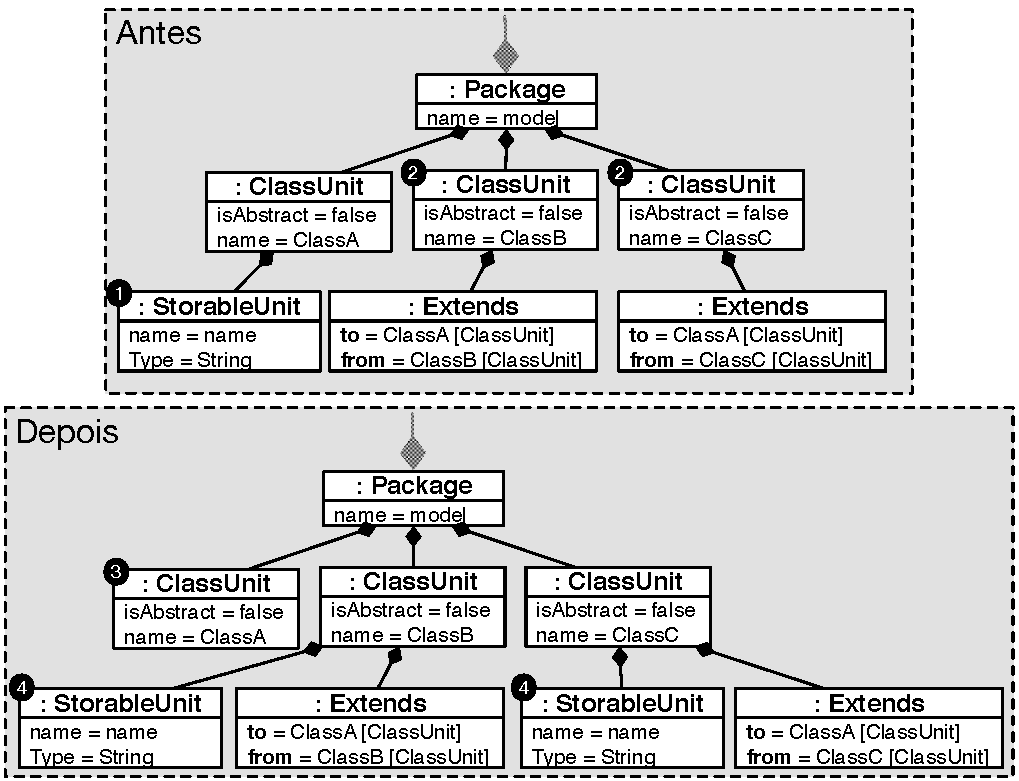
\includegraphics[scale=0.6]{images/pushDownStorableUnitAntesDepois2}
	\fautor
\end{figure}

\subsubsection{Implementar Operações}

Após identificar as operações que compõem a refatoração a ser criada, o próximo passo consiste na implementação das operações. O terceiro passo da abordagem é apoiado por um conjunto de \textit{templates} que auxilia o engenheiro de modernização a implementar as operações. As operações atômicas identificadas para implementar a refatoração \textit{Push Down Attribute} foram implementadas em ATL utilizando os \textit{templates} apresentados nos Códigos-fontes~\ref{codigo:template_addKDMElement} e~\ref{codigo:template_delete}. A combinação desses \textit{templates} resulta nos Códigos-fontes~\ref{codigo:push_Down_StorableUnit_ATL1} e~\ref{codigo:push_Down_StorableUnit_ATL2}.


\begin{codigo}[caption={[ATL representando a operação atômica \texttt{add}.] ATL representando a operação atômica \texttt{add}.},escapeinside={(*@}{@*)}, basicstyle=\footnotesize, label={codigo:push_Down_StorableUnit_ATL1}, language=ATL]{Name}
rule createStorableUnit {
	from
		source : MM!ClassUnit (source.name = (*@\aspas{\{sub-\texttt{ClassUnit}Selecionada\}}@*)
	to 
		target : MM!ClassUnit (
			codeElement(*@$\leftarrow$@*)source.codeElement(*@$\rightarrow$@*)including(newElement)
		),
		newElement: MM!StorableUnit (
			name(*@$\leftarrow$@*)(*@\{\texttt{StorableUnit}Selecionado.name\}@*)
		)
}
\end{codigo}

\begin{codigo}[caption={[ATL representando a operação atômica \texttt{delete}.] ATL representando a operação atômica \texttt{delete}.},escapeinside={(*@}{@*)}, basicstyle=\footnotesize, label={codigo:push_Down_StorableUnit_ATL2}, language=ATL]{Name}
rule deleteStorableUnit {
	from
		source : MM!StorableUnit (source.name = (*@\{\texttt{StorableUnit}Selecionado.name\}@*) and source.refImmediateComposite().name = (*@\{\texttt{ClassUnit}.name\}@*) )
	to
		drop
}
\end{codigo}

\subsubsection{Agrupar Operações}

Após implementar as operações atômicas seguindo os \textit{templates} apresentados neste capítulo, o próximo passo consiste em agrupar tais operações. Dessa forma, um \textit{template} para guiar o agrupamento das operações atômicas também foi definido neste capítulo (ver Código-fonte~\ref{codigo:template_module_agrupar}). O agrupamento das operações atômicas apresentadas nos Códigos-fontes~\ref{codigo:push_Down_StorableUnit_ATL1} e~\ref{codigo:push_Down_StorableUnit_ATL2} resulta na refatoração apresentada no Código-fonte~\ref{codigo:push_Down_StorableUnit_ATL}.

\begin{codigo}[caption={[ATL representando a refatoração \textit{Push Down Attribute}.] ATL da refatoração \textit{Push Down Attribute}.},escapeinside={(*@}{@*)}, basicstyle=\footnotesize, label={codigo:push_Down_StorableUnit_ATL}, language=ATL]{Name}
module pushDownStorableUnit;
create OUT : MM refining IN : MM;
rule createStorableUnit {
	from
		source : MM!ClassUnit (source.name = (*@\aspas{\{sub-\texttt{ClassUnit}Selecionada\}}@*)
	to 
		target : MM!ClassUnit (
			codeElement(*@$\leftarrow$@*)source.codeElement(*@$\rightarrow$@*)including(newElement)
		),
		newElement: MM!StorableUnit (
			name(*@$\leftarrow$@*)(*@\{\texttt{StorableUnit}Selecionado.name\}@*)
		)
}
rule deleteStorableUnit {
	from
		source : MM!StorableUnit (source.name = (*@\{\texttt{StorableUnit}Selecionado.name\}@*) and source.refImmediateComposite().name = (*@\{\texttt{ClassUnit}.name\}@*) )
	to
		drop
}
\end{codigo}

\subsubsection{Definir Restrições}

Após identificar as operações que compõem a refatoração e implementar a refatoração utilizando os \textit{templates} definidos na abordagem, o próximo passo consiste na definição de asserções (pré- e pós-condições) da refatoração. Para cada operação atômica identificada no segundo passo da abordagem, \textit{templates} são disponibilizados para auxiliar o engenheiro de modernização a criar tais asserções. No Código-fonte~\ref{codigo:precondicao_push_down_attribute}, é apresentada a pré-condição criada para a refatoração \textit{Push Down Attribute}, a qual foi criada usando uma combinação dos \textit{templates} apresentados nos Códigos-fontes~\ref{codigo:pre_template_add} e~\ref{codigo:pre_template_delete}. 


\begin{codigo}[caption={[Pré-condição da refatoração \textit{Push Down Attribute}.] Pré-condição da refatoração \textit{Push Down Attribute}.},escapeinside={(*@}{@*)}, basicstyle=\footnotesize, label={codigo:precondicao_push_down_attribute}, language=OCL]{Name}
context StorableUnit::preCond(newName: String)
pre : ClassUnit.allInstances->select(e : ClassUnit | a.name = (*@\aspas{\{sub-\texttt{ClassUnit}Selecionada\}}@*) and not StorableUnit.refImmediateComposite().codeElement(*@$\rightarrow$@*)exist (e : StorableUnit | e.name = newName) 
and ClassUnit.allInstances->select(e : ClassUnit | a.name = (*@\{\texttt{ClassUnit}.name\}@*)) and StorableUnit.refImmediateComposite().codeElement(*@$\rightarrow$@*)exist (e : StorableUnit | e.name = newName)
\end{codigo}

Similarmente, no Código-fonte~\ref{codigo:poscondicao_push_down_attribute2}, é apresentada a pós-condição criada para a refatoração \textit{Push Down Attribute}.

\begin{codigo}[caption={[Pós-condição da refatoração \textit{Push Down Attribute}.] Pós-condição da refatoração \textit{Push Down Attribute}.},escapeinside={(*@}{@*)}, basicstyle=\footnotesize, label={codigo:poscondicao_push_down_attribute2}, language=OCL]{Name}
context StorableUnit::preCond(newName: String)
post : ClassUnit.allInstances->select(e : ClassUnit | a.name = (*@\aspas{\{sub-\texttt{ClassUnit}Selecionada\}}@*) and StorableUnit.refImmediateComposite().codeElement(*@$\rightarrow$@*)exist (e : StorableUnit | e.name = newName) 
and ClassUnit.allInstances->select(e : ClassUnit | a.name = (*@\{\texttt{ClassUnit}.name\}@*)) and not StorableUnit.refImmediateComposite().codeElement(*@$\rightarrow$@*)exist (e : StorableUnit | e.name = newName)
\end{codigo}


\subsubsection{Documentar Refatoração}

Para os exemplos apresentados neste capítulo, escolheu-se especificar as refatorações criadas seguindo o \textit{template} apresentado na Seção~\ref{sec:template_refatoracao}.

\begin{enumerate}
	\item Especificação Informal:
		\begin{enumerate}
			\item Nome: \textit{Push Down Attribute};
			\item Definição:
			    \begin{itemize}
			        \item \texttt{StorableUnit}Selecionado - um atributo que será movido para subclasses;
			        \item \texttt{ClassUnit} - uma classe na qual o \{\texttt{StorableUnit}Selecionado\} é definido;
			        \item sub-\texttt{ClassUnit}Selecionadas - subclasses de \{\texttt{ClassUnit}\}.
			    \end{itemize}
			\item Objetivo: Mover um \{\texttt{StorableUnit}Selecionado\} para as \{sub-\texttt{ClassUnit}Selecionadas\}.
			\item Descrição (opcional): \{\texttt{StorableUnit}Selecionado\} é utilizada em apenas algumas subclasses.
			\item Pré-condição:
			    \begin{itemize}
			        \item \{\texttt{StorableUnit}Selecionado\} não existe nas sub-\texttt{ClassUnit}Selecionadas; 
			        \item \{\texttt{StorableUnit}Selecionado\} existe na \texttt{ClassUnit}. 
			    \end{itemize}
			\item Pós-condição:
			    \begin{itemize}
			        \item \{\texttt{StorableUnit}Selecionado\} existe nas sub-\texttt{ClassUnit}Selecionadas;
			        \item \{\texttt{StorableUnit}Selecionado\} não existe na \texttt{ClassUnit}.
			    \end{itemize}
			\item Mecanismo: move um atributo de uma classe para todas suas subclasses;
			\item Algoritmo: 
			    \begin{itemize}
			        \item para cada sub-\texttt{ClassUnit}Selecionadas que realmente usa o \{\texttt{StorableUnit}Selecionado\} - sub-\texttt{ClassUnit}Selecionadas.add(\{\texttt{StorableUnit}Selecionado\})
			        \item \{\texttt{ClassUnit}\}.delete(\{\texttt{StorableUnit}Selecionado\}). 
			    \end{itemize} 
	    \end{enumerate}
		\item Especificação Formal:
		\begin{enumerate}
			\item Pré-condição: a pré-condição da refatoração \textit{Push Down Attribute} é apresentada no Código-fonte~\ref{codigo:precondicao_push_down_attribute};
			\item Algoritmo: a ATL responsável por realizar a refatoração \textit{Push Down Attribute} é apresentada no Código-fonte~\ref{codigo:push_Down_StorableUnit_ATL}
			\item Pós-condição: a pós-condição da refatoração \textit{Push Down Attribute} é apresentada no Código-fonte~\ref{codigo:poscondicao_push_down_attribute2};
		\end{enumerate}
	\end{enumerate}		
	
	
	
%--------------------------
\subsection{Criar Refatoração \textit{Extract Class}}
A refatoração \textit{Extract Class} deve ser utilizada quando uma determinada classe está fazendo o trabalho que deveria ser realizado por duas classes~\cite{Fowler1999}. Dessa forma, nesta seção, a refatoração \textit{Extract Class} é criada seguindo todos os passos da abordagem. 

\subsubsection{Identificar Elementos Estruturais}

A refatoração \textit{Extract Class} basicamente consiste na criação de uma nova classe, e em sequência deve-se mover todos os atributos relevantes de uma classe para essa nova classe. Dessa forma, as construções da linguagem OO utilizadas na refatoração são: (\textit{i}) classes e (\textit{ii}) atributos. Utilizando o artefato apresentado na Tabela~\ref{tab:mapemanetoEntreOOPeKDM}, é possível identificar que as metaclasses em KDM que representam essas construções em OO são \texttt{ClassUnit} e \texttt{StorableUnit}, respectivamente.

\subsubsection{Identificar Operações}

No segundo passo da abordagem deve-se identificar as operações atômicas que compõem a refatoração a ser criada. Na Figura~\ref{fig:antes_e_depois_extract_ClassUnit}, são apresentadas duas instâncias simplificada do KDM, uma representa a instância antes da refatoração e a outra representa a instância após a aplicação da refatoração. 

\begin{figure}[h]
	\centering
	% Requires \usepackage{graphicx}
	\caption{Instância simplificada do KDM antes e depois da refatoração \textit{Extract Class}.}
	\label{fig:antes_e_depois_extract_ClassUnit}
	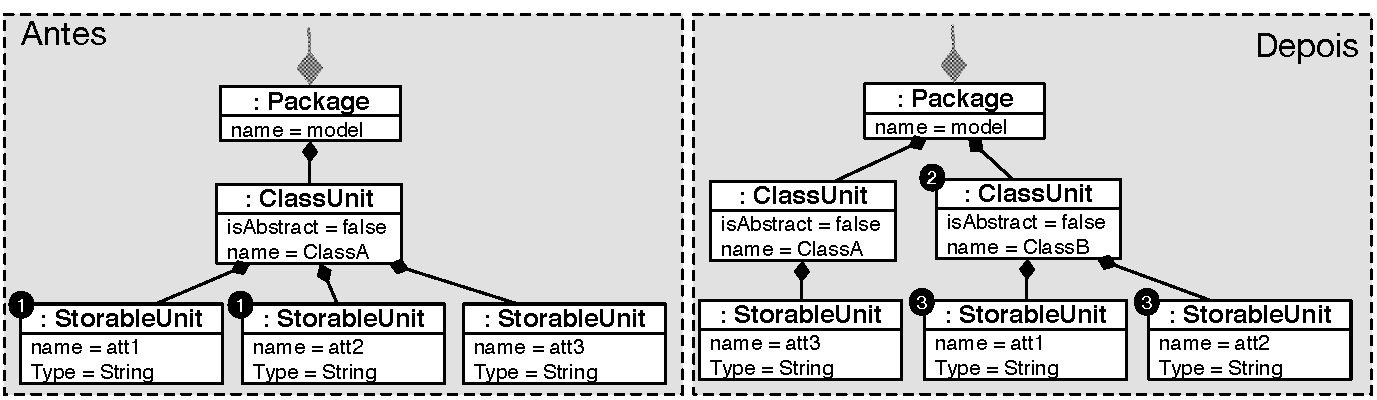
\includegraphics[scale=0.6]{images/extractClassUnitAntesEDepois2}
	\fautor
\end{figure}

O primeiro passo da refatoração \textit{Extract ClassUnit} é selecionar um conjunto de \texttt{StorableUnits} que será adicionado em uma nova instância de metaclasse \texttt{ClassUnit}, no exemplo ilustrado na Figura~\ref{fig:antes_e_depois_extract_ClassUnit} \ding{202}, duas instâncias de \texttt{StorableUnits} são selecionadas, \texttt{att1} e \texttt{att2}. Em seguida, uma instância da metaclasse \texttt{ClassUnit} é criada e adicionada ao mesmo \texttt{Package} que a instância da metaclasse \texttt{ClassUnit} e que contém os \{\texttt{StorableUnit}Selecionados\}, como ilustrado na Figura~\ref{fig:antes_e_depois_extract_ClassUnit} \ding{204}. Em seguida, todos \{\texttt{StorableUnit}Selecionados\} são adicionados nessa nova instância, como representado na Figura~\ref{fig:antes_e_depois_extract_ClassUnit} \ding{203}. Além disso, os \{\texttt{StorableUnit}Selecionados\} devem ser deletados da \{\texttt{ClassUnit}Selecionada\}. Observando a Figura~\ref{fig:antes_e_depois_extract_ClassUnit} é possível identificar que é a refatoração \textit{Extract Class} pode ser criada por meio da combinação das seguintes operações atômicas: (\textit{i}) \texttt{add} e (\textit{ii}) \texttt{delete}. 

%Mais especificadamente deve-se \texttt{add} uma instância de \texttt{ClassUnit}, \texttt{add} uma instância de \texttt{StorableUnit} na instância de \texttt{ClassUnit} criada e posteriormente deve-se \texttt{delete} 

\subsubsection{Implementar Operações}

No passo anterior identificou-se que as operações atômicas \texttt{add} e \texttt{delete} quando combinadas podem compor e criar a refatoração \textit{Extract Class}. Dessa forma, essas operações atômicas foram implementadas em ATL utilizando os \textit{templates} apresentados nos Códigos-fontes~\ref{codigo:template_addKDMElement} e~\ref{codigo:template_delete}. A combinação desses \textit{templates} resultou nos Códigos-fontes~\ref{codigo:extract_classUnit_ATL1}, ~\ref{codigo:extract_classUnit_ATL2} e~\ref{codigo:extract_classUnit_ATL3}. 

\begin{codigo}[caption={[ATL representando a operação atômica \texttt{add} \texttt{ClassUnit} da refatoração \textit{Extract ClassUnit}.] ATL representando a operação atômica \texttt{add} \texttt{ClassUnit} da refatoração \textit{Extract ClassUnit}.},escapeinside={(*@}{@*)}, basicstyle=\footnotesize, label={codigo:extract_classUnit_ATL1}, language=ATL]{Name}
rule createClassUnit {
	from
		source : MM!Package (source.name = (*@\aspas{\{\texttt{Package}\}}@*))
	to 
		target: MM!Package (
			codeElement(*@$\leftarrow$@*)source.codeElement(*@$\rightarrow$@*)including(newElement)
		),
		newElement: MM!ClassUnit (
			name(*@$\leftarrow$@*)(*@\aspas{\{newName\}}@*)
		)
}
\end{codigo}

\begin{codigo}[caption={[ATL representando a operação atômica \texttt{add} \texttt{StorableUnit} da refatoração \textit{Extract ClassUnit}.] ATL representando a operação atômica \texttt{add} \texttt{StorableUnit} da refatoração \textit{Extract ClassUnit}.},escapeinside={(*@}{@*)}, basicstyle=\footnotesize, label={codigo:extract_classUnit_ATL2}, language=ATL]{Name}
rule createStorableUnit {
	from
		source : MM!ClassUnit (source.name = (*@\aspas{\{newName\}}@*))
	to 
		target: MM!ClassUnit (
			codeElement(*@$\leftarrow$@*)source.codeElement(*@$\rightarrow$@*)including(newElement)
		),
		newElement: MM!StorableUnit (
			name(*@$\leftarrow$@*)(*@\aspas{storableUnitName}@*)
		)
}
\end{codigo}

\begin{codigo}[caption={[ATL representando a operação atômica \texttt{delete} \texttt{StorableUnit} da refatoração \textit{Extract ClassUnit}.] ATL representando a operação atômica \texttt{delete} \texttt{StorableUnit} da refatoração \textit{Extract ClassUnit}.},escapeinside={(*@}{@*)}, basicstyle=\footnotesize, label={codigo:extract_classUnit_ATL3}, language=ATL]{Name}
rule deleteStorableUnit {
	from
		source : MM!StorableUnit (source.name = (*@\aspas{\{StorableUnit\}Selecionado}@*) and source.refImmediateComposite().name = (*@\aspas{\{ClassUnit\}Selecionado}@*))
	to 
		drop
}
\end{codigo}

%Nas linhas 3-8 uma instância de \texttt{StorableUnit} é deletada. Nas linhas 9-19 uma instância da metaclasse \texttt{ClassUnit} é criada. Finalmente, nas linhas 14-24 uma instância da metaclasse \texttt{StorableUnit} é criada e adicionada na instância da metaclasse \texttt{ClassUnit} recém criada.

\subsubsection{Agrupar Operações}

Após implementar as operações atômicas seguindo os \textit{templates} apresentados neste capítulo, o próximo passo consiste em agrupar tais operações. Dessa forma, um \textit{template} para guiar o agrupamento das operações atômicas também foi definido neste capítulo (ver Código-fonte~\ref{codigo:template_module_agrupar}). O agrupamento das operações atômicas apresentadas nos Códigos-fontes~\ref{codigo:extract_classUnit_ATL1}, ~\ref{codigo:extract_classUnit_ATL2} e~\ref{codigo:extract_classUnit_ATL3} resulta na refatoração apresentada no Código-fonte~\ref{codigo:extract_classUnit_ATL}.

\begin{codigo}[caption={[ATL representando a refatoração \textit{Extract ClassUnit}.] ATL da refatoração \textit{Extract ClassUnit}.},escapeinside={(*@}{@*)}, basicstyle=\footnotesize, label={codigo:extract_classUnit_ATL}, language=ATL]{Name}
module extractClassUnit;
create OUT : MM refining IN : MM;
rule createClassUnit {
	from
		source : MM!Package (source.name = (*@\aspas{\{\texttt{Package}\}}@*))
	to 
		target: MM!Package (
			codeElement(*@$\leftarrow$@*)source.codeElement(*@$\rightarrow$@*)including(newElement)
		),
		newElement: MM!ClassUnit (
			name(*@$\leftarrow$@*)(*@\aspas{\{newName\}}@*)
		)
}
rule createStorableUnit {
	from
		source : MM!ClassUnit (source.name = (*@\aspas{\{newName\}}@*))
	to 
		target: MM!ClassUnit (
			codeElement(*@$\leftarrow$@*)source.codeElement(*@$\rightarrow$@*)including(newElement)
		),
		newElement: MM!StorableUnit (
			name(*@$\leftarrow$@*)(*@\aspas{storableUnitName}@*)
		)
}
rule deleteStorableUnit {
	from
		source : MM!StorableUnit (source.name = (*@\aspas{\{StorableUnit\}Selecionado}@*) and source.refImmediateComposite().name = (*@\aspas{\{ClassUnit\}Selecionado}@*))
	to 
		drop
}}
\end{codigo}

\subsubsection{Definir Restrições}

Após identificar as operações e implementar a refatoração, o próximo passo consiste na definição das pré- e pós-condições da refatoração. Os \textit{templates} apresentados neste capítulo foram utilizados para criar as asserções da refatoração \textit{Extract Class}. O Código-fonte~\ref{codigo:precondicao_extractClass} apresenta a pré-condição criada para a refatoração. Essa pré-condição foi criada utilizando os \textit{templates} apresentados nos Códigos-fontes~\ref{codigo:pre_template_add} e~\ref{codigo:pre_template_delete}. Similarmente, o Código-fonte~\ref{codigo:poscondicao_extractClass} apresenta a pós-condição criada para a refatoração \textit{Extract ClassUnit}.

\begin{codigo}[caption={[Pré-condição da refatoração \textit{Extract Class}.] Pré-condição da refatoração \textit{Extract Class}.},escapeinside={(*@}{@*)}, basicstyle=\footnotesize, label={codigo:precondicao_extractClass}, language=OCL]{Name}
context StorableUnit::preCond(newName: String)
pre : ClassUnit.allInstances->select(e : ClassUnit | a.name = (*@\{\texttt{ClassUnit}Selecionada\}@*)) and StorableUnit.refImmediateComposite().codeElement(*@$\rightarrow$@*)exist (e : StorableUnit | e.name = (*@\{\texttt{StorableUnit}Selecionado\}@*))
and Package.allInstances->select(e : Package | a.name = (*@\aspas{\{Package\}}@*) and not ClassUnit.refImmediateComposite().codeElement(*@$\rightarrow$@*)exist (e : ClassUnit | e.name = newName) 
and ClassUnit.allInstances->select(e : ClassUnit | a.name = newName and not StorableUnit.refImmediateComposite().codeElement(*@$\rightarrow$@*)exist (e : StorableUnit | e.name = (*@\{\texttt{StorableUnit}Selecionado\}@*).name) 
\end{codigo}

\begin{codigo}[caption={[Pós-condição da refatoração \textit{Extract ClassUnit}.] Pós-condição da refatoração \textit{Extract ClassUnit}.},escapeinside={(*@}{@*)}, basicstyle=\footnotesize, label={codigo:poscondicao_extractClass}, language=OCL]{Name}
context StorableUnit::preCond(newName: String)
post : ClassUnit.allInstances->select(e : ClassUnit | a.name = (*@\{\texttt{ClassUnit}Selecionada\}@*)) and not StorableUnit.refImmediateComposite().codeElement(*@$\rightarrow$@*)exist (e : StorableUnit | e.name = (*@\{\texttt{StorableUnit}Selecionado\}@*).name)
and Package.allInstances->select(e : Package | a.name = (*@\aspas{\{Package\}}@*) and ClassUnit.refImmediateComposite().codeElement(*@$\rightarrow$@*)exist (e : ClassUnit | e.name = newName) 
and ClassUnit.allInstances->select(e : ClassUnit | a.name = newName and StorableUnit.refImmediateComposite().codeElement(*@$\rightarrow$@*)exist (e : StorableUnit | e.name = (*@\{\texttt{StorableUnit}Selecionado\}@*).name) 
\end{codigo}

\subsubsection{Documentar Refatoração}

O último passo da abordagem é a especificação da refatoração criada. Esse passo é opcional e fica a critério do engenheiro de modernização realizar esse passo. Para a refatoração \textit{Extract ClassUnit} escolheu-se especificar a refatoração seguindo o \textit{template} apresentado na Seção~\ref{sec:template_refatoracao}.


\begin{enumerate}
	\item Especificação Informal:
		\begin{enumerate}
			\item Nome: \textit{Extract ClassUnit};
			\item Definição:
			    \begin{itemize}
			        \item \texttt{Package} - uma instância da metaclasse \texttt{Package} para adicionar a nova \texttt{ClassUnit};
			        \item \texttt{ClassUnit}Selecionada - a classe que contém os atributos e métodos que devem ser movido para a nova classe;
			        \item novoNome - um novo nome para a nova classe a ser criada;
			        \item \texttt{StorableUnit}Selecionado - atributo selecionado para ser movido para a nova classe.
			    \end{itemize}
			\item Objetivo: Criar uma nova \texttt{ClassUnit} e mover o \texttt{StorableUnit}Selecionado para essa nova instância.
			\item Descrição (opcional): \texttt{ClassUnit}Selecionada está realizando o trabalho que deveria ser realizado por duas classes.
			\item Pré-condição:
			    \begin{itemize}
			        \item \{\texttt{StorableUnit}Selecionado\} existe na \{\texttt{ClassUnit}Selecionada\};
			        \item nova \texttt{ClassUnit} não existe no \texttt{Package};
			        \item \{\texttt{StorableUnit}Selecionado\} não existe na nova \texttt{ClassUnit}.
			    \end{itemize}
			\item Pós-condição:
			    \begin{itemize}
			        
			        \item \{\texttt{StorableUnit}Selecionado\} não existe na \{\texttt{ClassUnit}Selecionada\};
			        \item nova \texttt{ClassUnit} existe no \texttt{Package};
			        \item \{\texttt{StorableUnit}Selecionado\} existe na nova \texttt{ClassUnit}.
			    \end{itemize}
			\item Mecanismo: Deve-se criar uma nova classe e mover os atributos selecionados;
			\item Algoritmo: 
			    \begin{itemize}
			        \item addNewClassUnit(\{novoNome\});
			        \item adiciona essa nova instância dentro de um \texttt{Package};
			        \item para cada \{\texttt{StorableUnit}Selecionado\} - add(\{newClassUnit\}, \{\texttt{StorableUnit}\-Selecionado\});
			        \item para cada \{\texttt{StorableUnit}Selecionado\} - delete(\{\texttt{ClassUnit}Selecionada\}, \{\texttt{Storable\-Unit}Selecionado\});
			        %\item createNewHasType(\{newClassUnit\}, \{\texttt{ClassUnit}Selecionada\}).
			    \end{itemize} 
	    \end{enumerate}
		\item Especificação Formal:
		\begin{enumerate}
			\item Pré-condição: a pré-condição da refatoração \textit{Extract Class} é apresentada no Código-fonte~\ref{codigo:precondicao_extractClass};
			\item Algoritmo: a ATL responsável por realizar a refatoração \textit{Extract Class} é apresentada no Código-fonte~\ref{codigo:extract_classUnit_ATL};
			\item Pós-condição: a pós-condição da refatoração \textit{Extract Class} é apresentada no Código-fonte~\ref{codigo:poscondicao_extractClass};
		\end{enumerate}
\end{enumerate}


\section{Trabalhos Relacionados}\label{sec:trabalhos_relacionados_abordagem_criar_kdm}

Nesta seção, são descritos os principais trabalhos encontrados na literatura que remetem às abordagens para a criação de refatorações em nível de modelos. De acordo com o mapeamento sistemático~\cite{durelli_systematic_mapping}, poucos trabalhos propuseram abordagens para criar refatorações em nível de modelo, entre eles, alguns não mostraram dados suficientes que pudessem ser utilizados nesta tese. Entretanto, foram identificados alguns trabalhos que deram suporte e guiaram o desenvolvimento da abordagem descrita neste capítulo, assim, nesta seção, são mostradas as principais semelhanças e diferenças encontradas entre eles.

~\citeonline{sen2012reusable} definem uma abordagem para especificar refatorações de forma genérica. Os autores apresentam um metametamodelo denominado \textit{GenericMT}, o qual contém elementos estruturais do POO (classes, métodos, atributos, parâmetros, etc.). Por meio desse metametamodelo, refatorações genéricas podem ser criadas. Para ativar as refatorações de forma genérica para um metamodelo específico, uma adaptação é necessária. Após a criação dessa adaptação, todas as refatorações criadas podem ser aplicadas em instâncias do metamodelo adaptado. A aplicação das refatorações é realizada utilizando os conceitos de entrelaçamento do paradigma orientado a aspectos. Uma limitação dessa abordagem é a estrutura do \textit{GenericMT}, pois apenas elementos estruturais do POO podem ser refatorados. Refatorações que necessitam de outros elementos estruturais para realizar a sua operação não podem ser criadas por meio dessa abordagem. Por outro lado, a abordagem apresentada neste capítulo permite que o engenheiro de modernização crie refatorações para diversos elementos estruturais, uma vez que o metamodelo KDM contém metaclasses para representar diversos artefatos de um sistema. Além disso, a abordagem definida por esses autores não utiliza metamodelos padronizados, tais como: UML e KDM. Os autores não deixam claro se as refatorações são apoiadas por diretrizes/passos. A abordagem apresentada aqui define um conjunto de seis passos para auxiliar o engenheiro de modernização a criar refatorações para o KDM, assim, \textit{templates} foram definidos. Da mesma forma que a abordagem destacada neste capítulo, ~\citeonline{sen2012reusable} também utilizam restrições (pré- e pós-condições) nas refatorações criadas.

Uma abordagem muito similar é proposta por~\citeonline{tichelaar2000meta}. Os autores introduzem uma abordagem que utiliza o metamodelo FAMIX, permitindo a criação de refatorações para elementos estruturais do POO (classes, objetos, métodos, etc.) e todas as refatorações criadas utilizam a ferramenta MOOSE~\cite{ducasse2005moose}. De acordo com os autores, tal abordagem é independente de linguagem, visto que MOOSE aceita como entrada as linguagens Java, C++ e Smalltalk. Porém, os autores não utilizam um metamodelo padronizado pelo OMG, FAMIX é um metamodelo proprietário, o que pode dificultar a interoperabilidade entre outros apoios ferramentais. Da mesma forma que a abordagem descrita aqui, os autores também utilizam operações atômicas (\texttt{add}, \texttt{delete} e \texttt{change}) para compor as refatorações criadas para o metamodelo FAMIX. Restrições também são suportadas na abordagem proposta por~\citeonline{tichelaar2000meta}.  


Seguindo a mesma linha de pensamento, outra abordagem foi proposta por~\citeonline{Zhang_2005}, a qual salienta que refatorações genéricas também são criadas por meio do \sigla{GME}{\textit{Generic Modeling Environment}}~\cite{ledeczi2001generic}. Essa abordagem utiliza instâncias do metamodelo UML e todas as refatorações genéricas são criadas para serem aplicadas em UML. Os autores utilizam o metamodelo UML, o qual é também padronizado pelo OMG. Similarmente a abordagem descrita neste capítulo, os autores também utilizam operações atômicas (\texttt{add}, \texttt{delete} e \texttt{change}) para compor as refatorações criadas para o metamodelo UML. Restrições também são definidas em OCL na abordagem proposta por~\citeonline{Zhang_2005}.  


%Diagrama de classe UML, além de ser o modelo mais utilizado durante o desenvolvimento de sistemas orientados a objeto, é também o diagrama mais utilizado para aplicar refatorações em nível de modelo. De acordo com~\citeonline{Tom_2008_2008}, a principal razão desse diagrama ser o mais utilizado para aplicar refatorações em nível de modelo é que o mesmo é muito similar as estrutural do POO. Assim, a maioria das abordagens e refatorações definidas em nível de programa podem ser diretamente aplicadas em diagramas de classe UML.

~\citeonline{brosch2009operation} definem uma abordagem que permite a especificação de refatorações em instâncias de qualquer metamodelo. Modificações realizadas nos metamodelos são armazenadas, abstraídas e, então, propagadas para manter o metamodelo sincronizado e consistente. As principais semelhanças com a abordagem descrita neste capítulo são: (\textit{i}) operações atômicas são utilizadas para criar a base para as refatorações e (\textit{ii}) tais operações são agrupadas para criar a refatoração. As principais diferenças são: (\textit{i}) os autores não definem passos para a criação das refatorações, (\textit{ii}) não utilizam um metamodelo padronizado pelo OMG como base, porém, os autores afirmam que a abordagem pode ser aplicada a qualquer metamodelo, (\textit{iii}) \textit{templates} não são utilizados para auxiliar a criação das refatorações e (\textit{iv}) não é evidente se linguagens de restrições são utilizadas nas refatorações. 

~\citeonline{sun2009model} apresentam uma abordagem similar, porém, diferentemente de~\citeonline{brosch2009operation}, modificações realizadas são armazenadas em uma instância concreta de um metamodelo, e, em seguida, a abordagem identifica padrões de transformações, os quais podem ser replicados em outras instâncias do metamodelo para manter sua consistência. As principais diferenças com a abordagem descrita neste capítulo são: (\textit{i}) os autores não especificam passos para conduzir o engenheiro de modernização durante a criação de refatorações, (\textit{ii}) da mesma forma que~\citeonline{brosch2009operation}, ~\citeonline{sun2009model} não utilizam um metamodelo padronizado pelo OMG como base, porém, os autores afirmam que a abordagem pode ser aplicada a qualquer metamodelo, (\textit{iii}) \textit{templates} também não são explicitamente citados na abordagem e (\textit{iv}) não é evidente se linguagens de restrições são utilizadas na abordagem. As principais semelhanças identificadas são: (\textit{i}) operações atômicas são utilizadas para criar as refatorações e (\textit{ii}) tais operações são agrupadas para criar a refatoração.  


%Essas abordagens são similares a abordagem descrita neste capítulo, visto que um módulo de sincronização (ver Capítulo~\ref{chapter:ferramenta_kdm_re}, Seção~\ref{sec:modulo_de_sincronizacao_kdm_re}) também foi desenvolvido, buscando deixar a instância do metamodelo KDM sincronizado e consistente após a aplicação de refatorações de forma automática.

~\citeonline{langer2010model} também apresentam uma abordagem para realizar transformações em modelos, a qual é denominada REMA e busca a derivação incremental de regras de transformação. Essas regras podem ser usadas para aplicar refatorações automaticamente em qualquer modelo. As principais semelhanças identificadas com a abordagem descrita neste capítulo são: (\textit{i}) operações atômicas são utilizadas, (\textit{ii}) operações compostas são criadas por meio da combinação de um conjunto de operações atômicas e, assim, as refatorações são criadas e (\textit{iii}) restrições também são utilizadas na abordagem proposta por~\citeonline{langer2010model}. As diferenças explicitamente identificadas com a abordagem apresentada neste capítulo são: (\textit{i}) nenhuma diretriz é apresentada para guiar a criação das refatorações, (\textit{ii}) os autores não utilizam metamodelo padronizados e (\textit{iii}) \textit{templates} também não são citados na abordagem.   


Similar à abordagem apresentada neste capítulo,~\citeonline{astels2002refactoring} define uma abordagem para aplicar refatorações em diagrama de classe da UML e suas refatorações são criadas por meio da combinação de operações atômicas (\texttt{add}, \texttt{delete}, etc.). Além disso, o autor também utiliza linguagem de transformação e OCL para definir as refatorações e suas restrições, respectivamente. Porém, nenhuma diretriz é apresentada na abordagem. Além disso, \textit{templates} também não são utilizados na abordagem. 

~\citeonline{Reimann_2015} define uma abordagem para criar e aplicar refatorações em nível de modelo de forma genérica. De acordo com o autor, sua abordagem pode ser aplicada em qualquer metametamodelo, metamodelo e modelo. Para isso, ele definiu um conjunto de passos e criou uma DSL, em que o usuário pode especificar a refatoração de forma independente e genérica. As principais semelhanças identificadas com a abordagem descrita neste capítulo são: (\textit{i}) os autores apresentam um conjunto de diretrizes para auxiliar o engenheiro a criar as refatorações, (\textit{ii}) operações atômicas também são utilizadas, (\textit{iii}) a composição dessas operações resulta na refatoração e (\textit{iv}) restrições são implementadas utilizando OCL. As diferenças são: (\textit{i}) da mesma forma que~\citeonline{brosch2009operation} e~\citeonline{sun2009model},  ~\citeonline{Reimann_2015} também não utiliza um metamodelo padronizado pelo OMG como base, porém, o autor afirma que a abordagem pode ser aplicada a qualquer metamodelo e (\textit{ii}) o autor não menciona a utilização de \textit{templates}.

~\citeonline{misbhauddin2012towards} descreve uma abordagem para aplicar refatorações em diversos diagramas da UML. Quando uma refatoração é aplicada, por exemplo, em um diagrama de classe, o efeito da refatoração é replicado em outros diagramas, tais como: diagrama de sequência, diagrama de caso de uso, etc. As principais semelhanças identificadas com a abordagem descrita neste capítulo são: (\textit{i}) o autor apresenta um conjunto de passos para auxiliar a criação de refatorações para um metamodelo padronização do OMG, nesse contexto, UML, (\textit{ii}) operações atômicas são utilizadas para criar as refatorações e (\textit{iii}) o autor utiliza linguagem de restrição escrita em OCL. As principais diferenças entre a abordagem proposta neste capítulo e a abordagem proposta por~\citeonline{misbhauddin2012towards} são: (\textit{i}) o autor não evidencia a utilização de \textit{templates} para criar as refatorações e (\textit{ii}) também não é evidente se as operações atômicas são agrupadas para criar refatorações mais complexas. 

Na Tabela~\ref{tab:relatedWorks_consideracoes_abordagem} é apresentada uma comparação entre a abordagem apresentada neste capítulo e os trabalhos relacionados quanto à forma como criam refatorações para modelos. Dessa forma, alguns critérios foram definidos durante a comparação, tais critérios são: (\textit{i}) a abordagem fornece diretrizes/passos; (\textit{ii}) a abordagem emprega o metamodelo KDM; (\textit{iii}) a abordagem disponibiliza \textit{templates}; (\textit{iv}) a abordagem considera operações atômicas; (\textit{v}) considera a composição de refatorações; e (\textit{vi}) a abordagem considera restrições. As colunas da tabela foram abreviadas, assim, \aspas{ATR} representa \aspas{Autor(es)}, \aspas{DRZ} representa \aspas{Diretrizes}, \aspas{TPT} representa \aspas{\textit{Templates}}, \aspas{OA} representa \aspas{Operações Atômicas}, \aspas{CR} representa \aspas{Composição de Refatoração} e \aspas{RTÇ} representa \aspas{Restrições}. O símbolo \aspas{\ding{51}} representa que a abordagem define o critério e o símbolo \aspas{\ding{55}} representa que a abordagem não define o critério.


\begin{table}[h]
\centering
\caption{Comparação entre a abordagem definida neste capítulo e os trabalhos relacionados.}
\label{tab:relatedWorks_consideracoes_abordagem}
\begin{tabular}{|l|l|l|l|l|l|l|}
\hline
\multicolumn{1}{|c|}{ATR} & DRZ & KDM & TPT & OA & CR & RTÇ \\ \hline
Durelli R. S. Capítulo~\ref{chapter:catalogo_refactoring_KDM}     &     \multicolumn{1}{c|}{\ding{51}}       & \multicolumn{1}{c|}{\ding{51}}    & \multicolumn{1}{c|}{\ding{51}}          &    \multicolumn{1}{c|}{\ding{51}}                &     \multicolumn{1}{c|}{\ding{51}}                       & \multicolumn{1}{c|}{\ding{51}}           \\ \hline
~\citeonline{sen2012reusable}&\multicolumn{1}{c|}{\ding{55}}&\multicolumn{1}{c|}{\ding{55}}&\multicolumn{1}{c|}{\ding{55}}&\multicolumn{1}{c|}{\ding{51}}&\multicolumn{1}{c|}{\ding{55}}&\multicolumn{1}{c|}{\ding{51}}\\ \hline
~\citeonline{tichelaar2000meta, ducasse2005moose}&\multicolumn{1}{c|}{\ding{55}}&\multicolumn{1}{c|}{\ding{55}}&\multicolumn{1}{c|}{\ding{55}}&\multicolumn{1}{c|}{\ding{51}}&\multicolumn{1}{c|}{\ding{51}}&\multicolumn{1}{c|}{\ding{51}}\\ \hline

~\citeonline{Zhang_2005}&\multicolumn{1}{c|}{\ding{55}}&\multicolumn{1}{c|}{\ding{55}}&\multicolumn{1}{c|}{\ding{55}}&\multicolumn{1}{c|}{\ding{51}}&\multicolumn{1}{c|}{\ding{51}}&\multicolumn{1}{c|}{\ding{51}}\\ \hline


~\citeonline{brosch2009operation}&\multicolumn{1}{c|}{\ding{55}}&\multicolumn{1}{c|}{\ding{55}}&\multicolumn{1}{c|}{\ding{55}}&\multicolumn{1}{c|}{\ding{51}}&\multicolumn{1}{c|}{\ding{51}}&\multicolumn{1}{c|}{\ding{55}}\\ \hline

~\citeonline{sun2009model}&\multicolumn{1}{c|}{\ding{55}}&\multicolumn{1}{c|}{\ding{55}}&\multicolumn{1}{c|}{\ding{55}}&\multicolumn{1}{c|}{\ding{51}}&\multicolumn{1}{c|}{\ding{51}}&\multicolumn{1}{c|}{\ding{55}}\\ \hline

~\citeonline{langer2010model}&\multicolumn{1}{c|}{\ding{55}}&\multicolumn{1}{c|}{\ding{55}}&\multicolumn{1}{c|}{\ding{55}}&\multicolumn{1}{c|}{\ding{51}}&\multicolumn{1}{c|}{\ding{51}}&\multicolumn{1}{c|}{\ding{51}}\\ \hline

~\citeonline{astels2002refactoring}&\multicolumn{1}{c|}{\ding{55}}&\multicolumn{1}{c|}{\ding{55}}&\multicolumn{1}{c|}{\ding{55}}&\multicolumn{1}{c|}{\ding{51}}&\multicolumn{1}{c|}{\ding{51}}&\multicolumn{1}{c|}{\ding{51}}\\ \hline

~\citeonline{Reimann_2015}&\multicolumn{1}{c|}{\ding{51}}&\multicolumn{1}{c|}{\ding{55}}&\multicolumn{1}{c|}{\ding{55}}&\multicolumn{1}{c|}{\ding{51}}&\multicolumn{1}{c|}{\ding{51}}&\multicolumn{1}{c|}{\ding{51}}\\ \hline

~\citeonline{misbhauddin2012towards}&\multicolumn{1}{c|}{\ding{51}}&\multicolumn{1}{c|}{\ding{55}}&\multicolumn{1}{c|}{\ding{55}}&\multicolumn{1}{c|}{\ding{51}}&\multicolumn{1}{c|}{\ding{55}}&\multicolumn{1}{c|}{\ding{51}}\\ \hline
\end{tabular}
\end{table}


\section{Considerações Finais}\label{sec:consideracoes_finais_capitulo_reforacao}

Neste capítulo, foram apresentados seis passos para auxiliar o engenheiro de modernização a criar refatorações para o metamodelo KDM. Com o intuito de exemplificar esses seis passos, foram escolhidas algumas refatorações propostas por~\citeonline{Fowler1999} para serem criadas para o metamodelo KDM. %Embora ~\citeonline{Fowler1999} tenha definido um catálogo de refatoração para ser utilizado em código-fonte, mais de 60\% das refatorações (44 de 72) são ilustradas e explicadas utilizando modelos, mais especificadamente diagramas de classes da UML. Esta observação fez com que tais refatorações fossem criadas para o metamodelo KDM. 

Antes de criar qualquer refatoração para o metamodelo KDM, o primeiro passo diz que é  necessário identificar as metaclasses do KDM que têm características similares aos conceitos do POO, bem como instruções comumente utilizadas em todas as linguagens de programação, tais como, ramificações, iterações, etc. Dessa maneira, esse capítulo também apresentou um mapeamento entre os conceitos do POO e o metamodelo KDM. Acredita-se que engenheiros de modernização pouco familiarizados com o metamodelo KDM podem gastar menos tempo durante a criação de novas refatorações com a utilização desse mapeamento, assim, qualquer exemplo de refatoração pode ser facilmente adaptado para o metamodelo KDM seguindo tal mapeamento, bem como os passos aqui apresentados.

Após identificar todos os elementos estruturais e identificar o mapeamento entre POO e o metamodelo KDM, o próximo passo é identificar quais operações compõem a refatoração que se almeja criar para o KDM. No contexto desta tese, todas as refatorações podem ser agrupadas em nível de granularidade. As granularidades podem ser definidas em dois níveis de operações: (\textit{i}) operação atômica e (\textit{ii}) operações compostas. As granularidades definidas como operações atômicas podem ser especificadas por meio de operações primitivas (\texttt{addd}, \texttt{delete} e \texttt{change}). As refatorações de granularidade compostas são uma combinação de operações atômicas (ver Tabela~\ref{tab:refatoringsCatalogo}). Em seguida, no próximo passo, o engenheiro de modernização deve implementar a refatoração por meio da linguagem de transformação ATL. Dessa forma, \textit{templates} foram criados para auxiliar os engenheiros de modernização a implementar refatorações utilizando a linguagem ATL. Posteriormente, o engenheiro de modernização deve implementar as restrições (pré- e pós-condições) da refatoração. Similarmente, \textit{templates} também foram definidos para auxiliar os engenheiros de modernização a criar as restrições para uma refatoração em nível do KDM.

Após criar uma determinada refatoração, bem como suas pré- e pós-condições para o metamodelo KDM, o engenheiro de modernização pode especificar e documentar a refatoração. Esse passo é opcional e fica a critério do engenheiro de modernização realizá-lo. Caso o engenheiro almeje documentar a refatoração duas especificações podem ser utilizadas: (\textit{i}) especificação informal e (\textit{ii}) especificação formal. Na primeira, a ideologia básica é permitir que o engenheiro de modernização expresse o propósito da refatoração por meio de linguagem natural. Na segunda, o engenheiro de modernização representa as pré- e pós-condições, bem como a transformação/refatoração propriamente dita em linguagens executáveis - OCL e ATL foram utilizadas, respectivamente. Ambas as especificações são úteis para o engenheiro de modernização, pois a especificação informal é utilizada para facilitar a compreensão e o propósito da refatoração e a especificação formal facilita a visualização da implementação da refatoração e suas asserções. Além disso, a especificação formal é de extrema importância para facilitar a automação das refatorações. %É importante destacar que neste capítulo apenas as refatorações \textit{Rename ClassUnit}, \textit{Pull Up StorableUnit}, \textit{Push Down StorableUnit} e \textit{Extract ClassUnit} são apresentadas e detalhadas.

Seguindo os passos apresentados neste capítulo, o engenheiro de modernização pode criar refatorações para o metamodelo KDM. No entanto, as especificações formais e informais resultantes não são suficientes para promover o reúso de refatorações no contexto do metamodelo KDM. Diante disso, no Capítulo~\ref{chapter:Toward_a_Refactoring_Metamodel_for_KDM} é apresentado um metamodelo para auxiliar o engenheiro de modernização a promover o reúso de refatorações no contexto do metamodelo KDM. Com a utilização desse metamodelo, informações (metadados) sobre refatorações podem ser reutilizadas de forma independente de linguagem e plataforma. %No Capítulo~\ref{chapter:Abordagem_de_sincronizacao} uma abordagem para manter instâncias do metamodelo KDM sincronizada e consistente após a aplicação de refatoração é apresentada. 
No Capítulo~\ref{chapter:ferramenta_kdm_re}, é apresentado um apoio computacional denominado KDM-RE. Esse apoio computacional é composto por três \textit{plug-ins} do Eclipse: (\textit{i}) o primeiro compreende um conjunto de \textit{Wizards} que apoia o engenheiro de software na aplicação das refatorações em diagramas de classe UML; (\textit{ii}) o segundo consiste em um apoio à importação e ao reúso de refatorações disponíveis no repositório; (\textit{iii}) o terceiro constitui um módulo de propagação de mudanças que permite manter modelos internos sincronizados do KDM; 
